\documentclass[a4paper, 12pt]{article}

\usepackage[utf8]{inputenc}
\usepackage[T1]{fontenc}
%\usepackage[french]{babel}
\usepackage{amsmath, amssymb}
\usepackage{amsthm}
\usepackage{graphicx}
\usepackage{tikz}
\usetikzlibrary{positioning}
\usepackage{hyperref}
\usepackage{geometry}
\geometry{margin=1in}

\title{A mathematical modelling of rheumatoid arthritis}
\author{F. Apparailly, P. Azerad, O. Bortolotti,  G. Courties,  O. Iosifescu, A. Parmeggiani. }
\date{\today}
\usepackage{authblk}
\renewcommand\Authands{, }

\author[1]{F. Apparailly}
\author[2]{P. Azerad}
\author[1]{O. Bortolotti}
\author[1]{G. Courties}
\author[2]{O. Iosifescu}
\author[3]{A. Parmeggiani}

\affil[1]{IRMB, UMR1183, Université de Montpellier and INSERM, France}
\affil[2]{IMAG, UMR5149, Université de Montpellier, France}
\affil[3]{L2C, UMR5221, Université de Montpellier, France}
\newtheorem{rem}{Remark}[section]
\newtheorem{theorem}{Theorem}[section]
\newtheorem{proposition}{Proposition}[section]
\newcommand{\keywords}[1]{%
  \par\noindent\textbf{Keywords : }#1
}

\begin{document}

\maketitle 
\begin{abstract}
We developed a mathematical model to describe the inflammatory dynamics 
during arthritis development and resolution, focusing on the interaction between three key immune cell populations 
within the joint, namely neutrophils (N), synovial sublining tissue-resident macrophages (SL-TRM, T),
 and circulating monocytes that are recruited into the inflamed joint and differentiate into monocyte-derived macrophages (MoMac, M).
An inflammatory signal (S), representing the response to an external arthritogenic stimulus, 
drives the recruitment and activation of neutrophils and Momac, while SL-TRM exert a regulatory and protective role.
We propose a minimal ordinary differential equation model of acute inflammatory response into a joint that couples an inflammatory signal S to the three cell populations (N, T, M) and incorporates recruitment, conversion, nonlinear self-limitation and mutual regulation.
 We showed that the equilibrium structure depends on three adimensional parameters A, B, C and derived a cubic equation characterizing nontrivial steady states.
We performed an analytical study of equilibria and their stability, and identified a bifurcation at A = 1 separating a disease-free regime from a sustained inflammatory state, 
and discussed conditions for multiple biological feasible steady states, consistent with transient or persistent inflammation. 
Numerical simulations illustrate typical transient dynamics under various scenarios. 
In conclusion, our model provides a framework to explore mechanisms underlying acute versus sustained joint inflammation and offers a basis for parameter estimation from experimental data, and future extensions toward evaluation of therapeutic strategies.

\end{abstract}
\keywords{Arthritis;  Bifurcation Analysis; Inflammation; Persistence.}

\section{Introduction}
Mathematical modelling of  auto-immune disease is relatively recent.
According to the systematic survey on mathematical modelling of auto-immune disease by  Ugolkov et. al. \cite{frontiers2024},
the first papers date back to the 1970s. Since
then, the number of relevant articles increased exponentially,
reaching more than 200 publications per year by 2024. 
However according to Macfarlane et. al. \cite{macfarlane2020} which provides another careful and exhaustive bibliography in 2020, the number of  mathematical models of Rheumatoid Arthritis (RA) is still relatively small.
An illuminative survey paper introducing the issues and pitfalls of mathematical modelling in immunology is Andrew et. al.  \cite{andrew}. 
We refer to Handel et. al. \cite{Handel2020} for  examples and guidelines for sound mathematical modelling in immunology and also for the free software R-package DSAIRM \cite{dsairm2019} which allows to easily simulate and analyze a large variety of mathematical models of immune response.
Among mathematical models that deal with aspects
of RA, we can mention the following ones.
In Seymour et. al. \cite{seymour2001} a 4 equations model is introduced to describe the dynamics of the population of monocytes and the concentrations of three cytokines, namely IL-6, TNF-$\alpha$ and IL-10. 
In Jit et. al.  \cite{jit2005} RA vs. systemic inflammatory response syndrom is modelled by a system of four differential equations, describing the evolution of population of certain cell compartments, namely TNF-$\alpha$ (free or bound), antibodies and antibody-antigen complexes.
The effect of TNF-$\alpha$ inhibitors like (s)TNFR2, Etanecerp, Infliximab are investigated.
Baker et al.\cite{baker2013} introduced a model with pro-inflammation 
(p) and anti-inflammation cells (a) and considered a system of two differential equations for p and a. More complex models exhibiting various types of  bifurcations are introduced in \cite{baker2017}. 
In Odisharia et. al. \cite{jaiani2019} a 5 differential equations system is investigated to simulate the effect of tocilizumab on the populations of B and T-lymphocytes and cell population of cartilage.  
There exist also spatialized models, see Friedman et. al. \cite{friedman} where PDE (partial differential equations) are used to model a joint (synovial fluid and cartilage) and  Macfarlane et. al. \cite{macfarlane2022}
 where an hybrid model is introduced to describe pannus formation in a joint.
Effects of drugs such as infliximab, which blocks TNF-$\alpha$ ; methotrexate
which increases apoptosis of macrophages, and tocilizumab
which blocks the receptor of IL-6 are investigated.
In Relouw et. al. \cite{relouw} a 15 equations model with 48 parameters is introduced to model sepsis.
In Zhou et. al. \cite{zhou2018} a 4 differential equations model is introduced to describe the dynamics of the population of macrophages and fibroblasts cells and their mutual growth factor.
A paper that particularly inspired us 
is Ciuperca et. al. \cite{torres2024} which focus on Alzheimer disease and presents a minimal compartment model with  5 equations describing the concentrations of 
 A$\beta$-oligomers,
oligomers in the amyloid plaques,
A$\beta$-monomers,
microglial cells, and
interleukins.

Here we chose a compromise between simplicity and accuracy   to catch essential features. We chose to focus on cell populations and their interactions instead of the fine description of the many cytokines dynamics involved. Specifically, our model, presented in the next section, has 4 equations and only 7 parameters and is an ordinary differential equations systems. The behavior of the system will be shown to depend on a single nondimensional parameter.
Despite its simplicity (or due to) we hope that it can bring some understanding of the arthritis process and new ideas for therapy.\par
The paper is organized as follows.
In Section \ref{sec:model} we present the model discussed in the paper. In Section \ref{sec:analysis} we analyse the mathematical properties of the differential system, compute its steady states and discuss their stability. In Section \ref{sec:numerical_simulations}, we present some numerical simulations pertaining to different scenarii.
The paper ends with  Section \ref{sec:conclusion} concluding remarks and future work perspectives.


\section{Model}\label{sec:model}
In the experimental mouse model of arthritis used in this study,
 the acute inflammatory response is triggered by an external signal (injection of an arthritogenic serum) 
 that activates the immune system and initiates an inflammatory response 
 within the joint tissue, which is composed of a lining and sub-lining membrane.
  At steady state, the synovial lining membrane is populated by specialized tissue-resident macrophages (L-TRM) 
  that form a protective barrier and contribute to immune regulation. Tissue-resident macrophages (TRM) are also present within the sublining membrane (SL-TRM),
   scattered and fewer in number. 
  Both TRM contribute to early immune sensing of environmental cues, exerting an overall protective and regulatory role by limiting excessive inflammation.
   However, during arthritis inflammatory flares, while L-TRM remain preserved, SL-TRM. are progressively depleted. 
   This depletion is concomitant with the accumulation of macrophages derived from blood monocytes infiltrating the inflamed joints (Momac). 
   The loss of the SL-TRM population weakens synovial immune regulation and favors persistent inflammatory cell infiltration through 
   to the local production of cytokines and chemokines. This activation promotes the rapid recruitment of neutrophils (N) from the bloodstream into the joint, 
   where they become the dominant cell population during the acute phase of inflammation.
    Neutrophils amplify the inflammatory response through the release of pro-inflammatory mediators. 
     Based on these biological observations, we modeled the joint inflammatory response as the interaction between an inflammatory signal and three cell populations—N, SL-TRM, and Momac—capturing recruitment,
      amplification, and regulatory mechanisms in a minimal dynamical framework.



%Basically the crisis scenario is the following:
%The arthritis crisis is triggered by an external signal (injection of immune serum containing antigens) that activates the immune system and provokes an inflammatory response. 
%The antigens are recognized by the macrophages L-TRM (lining tissue resident macrophages) cells that secrete inflammatory chemokines and cytokines. 
%These cytokines activate the fibroblasts which in turn recruit the neutrophiles cells from the blood stream into the joint. 
%The cytokines also recruit the Momac cells from the blood stream into the joint. There is a positive feedback since the inflammation is amplified by the neutrophiles that are recruited in the joint by the chemokines secreted by the Momac cells. 
%The macrophages SL-TRM cells have a protective role since they inhibit the inflammation but they are depleted during the crisis because they are inhibited by the proliferation of Momac cells.
\subsection{Mathematical Model}
% explain the model when S=0 with the usual logistic growth of the cell populations, and then explain the effect of the inflammation on the recruitment and proliferation of the cells.
%explain the effect of the cells on the inflammation and the feedback loop between the inflammation and the cell populations.
The variable $S(t)$ is the inflammatory signal at time $t$. We take as unity the standard dose of the arthritogenic serum, so that $S(t)$ is dimensionless and represents the relative strength of the inflammatory signal with respect to the standard dose.
We rescale all variables by their respective baseline values in the disease-free state, so that they are dimensionless and represent relative populations with respect to their baseline levels.
Namely variable $N(t)$ (resp. $M(t)$, $T(t)$) designates the relative population of neutrophils (resp. Momac cells, SL-TRM cells) at time $t$ with respect to the baseline population $\widehat{N}$ (resp. $\widehat{M}$, $\widehat{T}$).\\
The cells $T$ (SL-TRM) and $M$ (Momac) interact with each other in the following way.
The Momac cells $M$ are recruited from the blood stream at a  rate $\beta S$ proportional to the inflammatory signal. They die at a rate $\delta_M\, M(M-1)$ and they transform into SL-TRM cells at a rate $\delta_M$. The SL-TRM cells $T$ die at a rate $\delta_M M$. 

The inflammatory state $S(t)$ is enhanced by neutrophils $N$ and inhibited by SL-TRM macrophages $T$.

Inflammation further increases neutrophils (factor $\alpha$), increases Momac (factor $\beta$), and decreases SL-TRM (factor $\gamma$).

Notice that we do not keep track of the population of fibroblasts, but rather the population of neutrophils, which are recruited by inflammatory chemokines.\\
The model is given by the following system of ordinary differential equations:

\begin{equation}
\left\{
\begin{aligned}
\frac{dS}{dt} &= (a\, N - b\,T) S \\
\frac{dN}{dt} &= \alpha S N - \delta_N N (N-1) \\
\frac{dM}{dt} &= \beta S - \delta_M M (M-1) \\
\frac{dT}{dt} &= -\gamma S T + \delta_M M (1-T)
\end{aligned}
\right.
\label{eq:system}
\end{equation}

where $a,b,\alpha,\beta,\gamma, \delta_N, \delta_M$ are positive parameters.
\begin{rem}
The term $\delta_M M (1-T)$ in the equation for $T$ models the conversion of Momac cells into SL-TRM cells, which is supported by experimental evidence.
Note that we could have add another parameter $\delta_T\neq \delta_M$ in this equation for $T$, but we choose to keep it simple since it did not change the dynamics of the crisis.
To make things easier to undestand, we summarize the model in the following diagram (see figure \ref{fig:graphe}).
\end{rem}

\usetikzlibrary{decorations.markings}
\tikzset{
    mid arrow/.style={
        decoration={markings, mark=at position 0.5 with {\arrow{>}}},
        postaction={decorate}
    },
    mid bar/.style={
        decoration={markings, mark=at position 0.5 with {\arrow{|-}}},
        postaction={decorate}
    }
}
% Usage examples (adapt to your existing \draw lines):
% \draw[mid arrow, thick] (N) to[bend left=20] (S);
% \draw[mid bar, thick]   (T) to[bend left=20] (S);
\begin{figure}[htb!]
\begin{center}
    \begin{tikzpicture}[node distance=4cm, auto, >=latex, thick]

        % Compartiments
        \node[draw, rectangle, fill=red!10, minimum width=3cm, minimum height=1cm] (N) {Neutrophils $N$};
        \node[draw, rectangle, fill=green!10, minimum width=3cm, minimum height=1cm, right=of N] (M) {Momac $M$};
        \node[draw, rectangle, fill=magenta!10, minimum width=3cm, minimum height=1cm, right=of M] (T) {SL-TRM $T$};
        \node[draw, circle, fill=blue!10, minimum size=2cm, below=of M, yshift=-1cm] (S) {Immune signal $S$};

        % Flèches et labels
        \draw[mid arrow, line width=1.5pt] (N) to[bend left=20] node[left, xshift=-2mm, yshift=2mm] {foster $(a)$} (S);
        \draw[dashed,-|, line width=1.5pt] (T) to[bend left=20] node[right, xshift=2mm] {inhibition $(b)$} (S);
        \draw[mid arrow, line width=1.5pt] (S) to[bend left=20] node[left] {activation$(\alpha)$} (N);
        \draw[mid arrow, line width=1.5pt] (S) to[bend left=10] node[left,xshift=6mm] {activation $(\beta)$} (M);
        \draw[dashed, line width=1.5pt, -|] (S) to[bend left=20] node[left, xshift=2mm] {inhibition $(\gamma)$} (T);
        \draw[dashed,-|, line width=1.5pt, loop above, looseness=8] (N) to node[above] {destruction $(\delta_N)$} (N);
        \draw[dashed,-|, line width=1.5pt, loop above, looseness=8] (M) to node[above] {destruction $(\delta_M)$} (M);
        \draw[mid arrow, line width=1.5pt] (M.east) -- node[below, yshift=-2mm] {conversion $(\delta_M)$} (T.west);

    \end{tikzpicture}
\end{center}
\label{fig:graphe}
\caption{Schematic representation of the model}
\end{figure}

\bigskip

%\textbf{Comments and questions on the model:}
%\marginpar{\textcolor{red}{\small to be completed by immunologists collaborators}}



\section{Analysis of the model}\label{sec:analysis}
\subsection{Existence and non-negativity of the solution.}
Existence and uniqueness of a local solution of the system \eqref{eq:system} is guaranteed by the Cauchy-Lipschitz theorem since the right-hand side of the system is locally Lipschitz continuous.
\begin{proposition}
If the initial conditions $S(0)$, $N(0)$, $M(0)$, and $T(0)$ are nonnegative, then the solution $(S(t), N(t), M(t), T(t))$ of the system \eqref{eq:system} remains nonnegative for all $t \geq 0$.   
\end{proposition}
\begin{proof}
We consider the vector field $F=(f_1, f_2, f_3, f_4)$ for $y=(y_1, y_2, y_3, y_4)\in \mathbb{R}^4$ given by:
\begin{equation*}
  \left\{
\begin{aligned}
f_1(y) &= (a y_2 - b y_4) y_1, \\
f_2(y) &= \alpha y_1 y_2 - \delta_N y_2 (y_2 - 1), \\
f_3(y) &= \beta y_1 - \delta_M y_3 (y_3 - 1), \\
f_4(y) &= -\gamma y_1 y_4 + \delta_M y_3 (1 - y_4).
\end{aligned}
\right.
\end{equation*}
We observe that the vector field $F$ is \emph{quasi-positive}, i.e. for each $i=1,2,3,4$, we have $f_i(y) \geq 0$ whenever $y_i = 0$ and $y_j \geq 0$ for all $j \neq i$. Thus from Proposition 2.1 in \cite{haraux2016}, we deduce that if the initial conditions are nonnegative, then the solution remains nonnegative for all $t \geq 0$.
\end{proof}
This property is biologically meaningful since the variables $S$, $N$, $M$, and $T$ represent cell populations, which cannot be negative. Our model thus ensures that the solutions remain within the biologically relevant domain.       
\subsection{Boundedness of the solution.}
Considering the equation for $T$, one can easily prove that $T(t)$  is always bounded by its initial value $T(0)$ or by 1 if $T(0) \leq 1$, for all $t \geq 0$. 
\begin{rem}This is biologically relevant since the population of SL-TRM cells is limited by spatial constraints within the joint tissue and regulatory mechanisms that control their proliferation.
\end{rem}
\marginpar{\textcolor{red}{\small is it biological fact that SL-TRM is bounded by disease-free value?}}

\begin{proposition}
Assume that the initial condition $T(0)$ is less than or equal to 1, then
the variable $T(t)$ is bounded by 1 for all $t \geq 0$. 
If $T(0) > 1$, then $T(t)$ is bounded by $T(0)$ for all $t \geq 0$.
%If $S(t)\to 0$ as $t\to +\infty$, then $T(t)\to 1$ as $t\to +\infty$.
%If $S(t)\to +\infty$ as $t\to +\infty$, then $T(t)\to 0$ as $t\to +\infty$.
\end{proposition}
\begin{proof}
    Let us consider the equation for $T$:
\begin{equation*}
\frac{dT}{dt} = -\gamma S T + \delta_M M (1 - T)
\end{equation*}
%If for some $t_0 >0$, we have $T(t_0) = 1$, then we have $1 - T(t_0) = 0$, hence $\delta_M M (1 - T) = 0$. Since $-\gamma S T \leq 0$, we deduce that $\frac{dT}{dt} \leq 0$ whenever $T(t) = 1$. Thus, if the solution starts with $T(0) \leq 1$, it cannot cross the threshold $T=1$ and must remain bounded by 1 for all time.
%In the other case, if $T(0) > 1$, then we have $1 - T(0) < 0$, hence $\delta_M M (1 - T(0)) \leq  0$. Since $-\gamma S T \leq 0$, we deduce that $\frac{dT}{dt} \leq  0$ at $t=0$. Thus, the solution will decrease and cannot exceed its initial value $T(0)$ for all time.    
Let us recall Gronwall's lemma: if $u(t)$ is a function satisfying the differential inequality
\begin{equation*}
\frac{du}{dt} \leq \alpha(t) u(t)
\end{equation*}
for some function $\alpha(t)$, then we have
\begin{equation*}
u(t) \leq u(0) \exp{\int_0^t \alpha(s) ds}.
\end{equation*}
If $T(0) \leq 1$, we can write the equation for $T-1$ as
\begin{equation*}
\frac{d(T-1)}{dt} = -\gamma S (T-1) - \delta_M M (T-1) -\gamma S 
\leq (-\gamma S - \delta_M M) (T-1)
\end{equation*}
Thus, by Gronwall's lemma, we have
\begin{equation*}
T(t) - 1 \leq (T(0) - 1) \exp{\int_0^t (-\gamma S(s) - \delta_M M(s)) ds} \leq 0
\end{equation*}
which proves that $T(t) \leq 1$ for all $t \geq 0$.\\
In the other case, if $T(0) > 1$, we can write the equation for $T - T(0)$ as
\begin{equation*}
\frac{d(T - T(0))}{dt} = -\gamma S (T - T(0)) - \delta_M M (T - T(0)) + \delta_M M (1 - T(0)) - \gamma S T(0) \leq (-\gamma S - \delta_M M) (T - T(0))
\end{equation*}
Thus, by Gronwall's lemma, we have
\begin{equation*}
T(t) - T(0) \leq (T(0) - T(0)) \exp{\int_0^t (-\gamma S(s) - \delta_M M(s)) ds} = 0
\end{equation*}
which proves that $T(t) \leq T(0)$ for all $t \geq 0$.  
\end{proof}
About the variables $S$, $N$ and $M$, we did not  include degradation terms in the $S$, $N$ and  $M$ equations, which could ensure the boundedness of $S$, $N$ and $M$.
    Indeed we shall see in Section \ref{sec:numerical_simulations} that in some cases the solution may not be bounded for all time, at least for $S$, $N$ and $M$.
     Actually we are interested in the  immune response to an external stimulus, which can lead to a very high level of inflammation and cell recruitment from the bloodstream or marrow. 
     The transient dynamics of the system can involve large variations in the levels of inflammation and cell populations, which may be shadowed by a model that includes degradation terms that dampens the growth of these variables.
    In our model, the solution may not be bounded for all time,
     but it can still be biologically relevant since we are interested in the early crisis dynamics 
     rather than the long-term behavior of the system.\\
However, we can still derive some lower bounds for the variables $M$ and $N$.    
Using Gronwall's lemma like in the previous proof, we can also bound from below the variables $M$ and  $N$.
\begin{proposition}
Assume that the initial condition $M(0)$ (resp. $N(0)$) is greater than or equal to 1, then
the variable $M(t)$ (resp. $N(t)$) is greater than or equal to 1 for all $t \geq 0$. If $M(0) < 1$ (resp. $N(0) < 1$), then $M(t)$ (resp. $N(t)$) is greater than or equal to $M(0)$ (resp. $N(0)$) for all $t \geq 0$.    
\end{proposition}
\begin{rem}
The upper boundedness of $T$ and the lower bounds for $M$ and $N$ are biologically relevant since they reflect the regulatory mechanisms that control the populations of SL-TRM, Momac, and neutrophils within the joint tissue. The population of SL-TRM cells is limited by spatial constraints and regulatory feedback, while the populations of Momac and neutrophils cannot fall below certain levels due to their large supply in blood and marrow.
\end{rem}
\marginpar{\textcolor{red}{\small is it biologically correct?}}

\subsection{Equilibria points}
\emph{Equilibria points} of the system are found by setting the right-hand side of the system to zero, i.e.
 the equilibrium points $(S^*, N^*, M^*, T^*)$ satisfy the following system of algebraic equations:
\begin{align}
(a N^* - b T^*) S^* &= 0 \label{eq:equilibrium_S} \\
\alpha S^* N^* - \delta_N N^* (N^* - 1) &= 0 \label{eq:equilibrium_N} \\
\beta S^* - \delta_M M^* (M^* - 1) &= 0 \label{eq:equilibrium_M} \\
-\gamma S^* T^* + \delta_M M^* (1 - T^*) &= 0 \label{eq:equilibrium_T}
\end{align}
\subsubsection{Inflammation free equilibria ($S^* =0$).}
A first natural equilibrium point is given by $S^* = 0, N^* = 1, M^* = 1, T^* = 1$. This point corresponds to the disease-free state, where there is no inflammation ($S^* = 0$) and the populations of neutrophils, Momac, and SL-TRM are at their baseline    levels ($N^* = 1, M^* = 1, T^* = 1$).

There are other equilibria points with $S^* = 0$  namely
$S^* = 0, N^* = 0, M^* = 0, T^* = R$, with arbitrary $R$;
 $S^* = 0, N^* = 0, M^* = 1, T^* = 1$;
 $S^* = 0, N^* = 1, M^* = 0, T^* = R$, with arbitrary $R$.
\begin{rem}
These equilibria points with  $N^* = 0$ or $M^* = 0$ are not biologically relevant since they correspond to the absence of neutrophils or Momac cells, which is not realistic in a living organism.
Furthermore, we will prove later that these equilibria points are unstable, so they will not be observed in physiological conditions.
\end{rem}

% Commented-out derivation for equilibria with S^* \neq 0
%For equilibria points with $S^* \neq 0$, from equation \eqref{eq:equilibrium_S} we have $a N^* - b T^* = 0$, hence 
%Therefore $\alpha S^* - \delta_N (N^* - 1) = 0$, so we can express $S^*$ in terms of $N^*$:
%\begin{equation}
%S^* = \frac{\delta_N}{\alpha} (N^* - 1)
%\label{eq:S_in_terms_of_N}
%\end{equation}
%We substitute \eqref{eq:T_in_terms_of_N}-\eqref{eq:S_in_terms_of_N}  into equation \eqref{eq:equilibrium_M} and \eqref{eq:equilibrium_T} and obtain a 2 by 2 system for  $M^*$ and  $N^*$:
%By substituting $T^* = \frac{a}{b} N^*$ and $S^* = \frac{\delta_N}{\alpha}(N^* - 1)$ into the equilibrium equations for $M^*$ and $T^*$, we obtain the following system for $N^*$ and $M^*$:
%\[
%\left\{
%\begin{aligned}
%&\beta \frac{\delta_N}{\alpha}(N^* - 1) - \delta_M M^* (M^* - 1) = 0 \\
%&-\gamma \frac{\delta_N}{\alpha}(N^* - 1) \cdot \frac{a}{b} N^* + \delta_M M^* \left(1 - \frac{a}{b} N^*\right) = 0
%\end{aligned}
%\right.
%\]
%This system allows us to determine the equilibrium values $N^*$ and $M^*$ when $S^* \neq 0$.
%Indeed we can express $N^*$ in terms of $M^*$ from the first equation:
%\begin{equation}
%N^* = 1 + \frac{\alpha \,\delta_M}{\beta \,\delta_N} M^* (M^* - 1)
%\label{eq:N_in_terms_of_M}
%\end{equation}
%Substituting this expression for $N^*$ into the second equation, we obtain an equation for $M^*$:
%\begin{equation}
%    M^* = \frac{a \,\gamma \,\delta_N}{b\, \alpha \,\delta_M} \frac{N^* (N^* - 1)}{(1 - \frac{a}{b} N^*)}
%    \label{eq:M_in_terms_of_N}
%\end{equation}
%Geometrically, the equilibria points with $S^* \neq 0$ correspond to the intersection points of the parabola defined by equations \eqref{eq:N_in_terms_of_M} and  the hyperbola defined by equation \eqref{eq:M_in_terms_of_N} in the $(N^*, M^*)$ plane. The number of such intersection points (and hence the number of equilibria with $S^* \neq 0$) depends on the parameters of the model.
%Substituting \eqref{eq:N_in_terms_of_M} into \eqref{eq:M_in_terms_of_N}, we  would obtain a quartic equation in $N^*$, which we do not write explicitly here due to its complexity.
%From basic algebra, we can show that there are at most 4 such intersection points, hence at most 4 equilibria points with $S^* \neq 0$. 
%We can be more precise because the biological feasibility imposes the roots to be real nonnegative numbers.
%Due to the structure of the irreducible  polynomial on $\mathbb{R}$ we can have either 0, or 2, or 4 real roots.
%We can find the asymptotes of the hyperbola and the apex of the parabola to determine the possible number of intersection points in the first quadrant.
%We rewrite the equation  \eqref{eq:M_in_terms_of_N} of the hyperbola as follows:
%\begin{equation}
%M^*= -\frac{\gamma \delta_N}{\alpha \delta_M}  (N^* + b/a -1) + \frac{(b/a)^{2}(1-b/a)}{(N^* - b/a)} 
%\label{eq:hyperbola_rewritten}
%\end{equation}
%From this expression, we see that the hyperbola has a vertical asymptote at $N^* = b/a$ and an oblique asymptote $M^* = -\frac{\gamma \delta_N}{\alpha \delta_M} (N^*+ b/a - 1)$.
%The parabola  \eqref{eq:N_in_terms_of_M} is horizontal in the $N,M$ plane, has its apex at  $N_{min} = 1 - \frac{\alpha \,\delta_M}{4 \beta \,\delta_N}$ and $M=1/2$ and is symmetric with respect to the horizontal line $M = 1/2$ and opens eastwards.
%We plot some typical cases in the following figure.


%\begin{figure}[htbp]
%    \centering
%    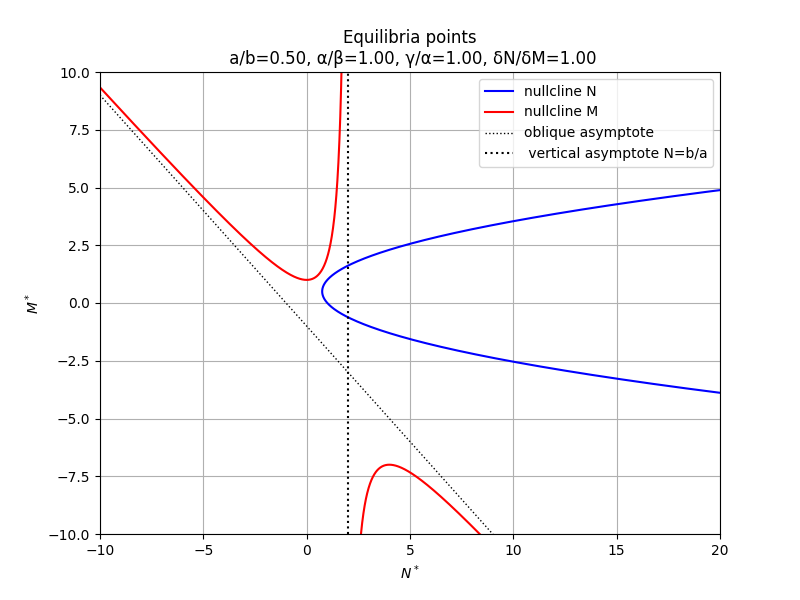
\includegraphics[width=0.45\textwidth]{equilibres.png}
%    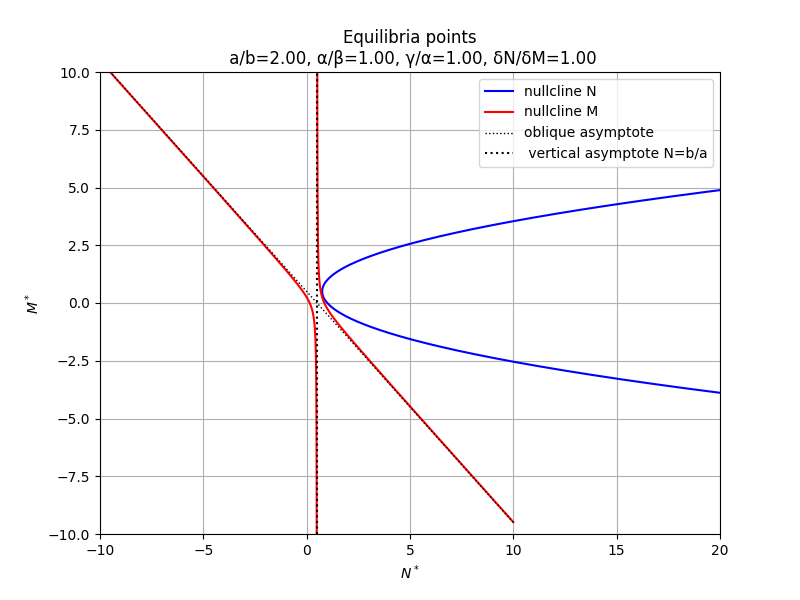
\includegraphics[width=0.45\textwidth]{equilibres_1.png}\\
%    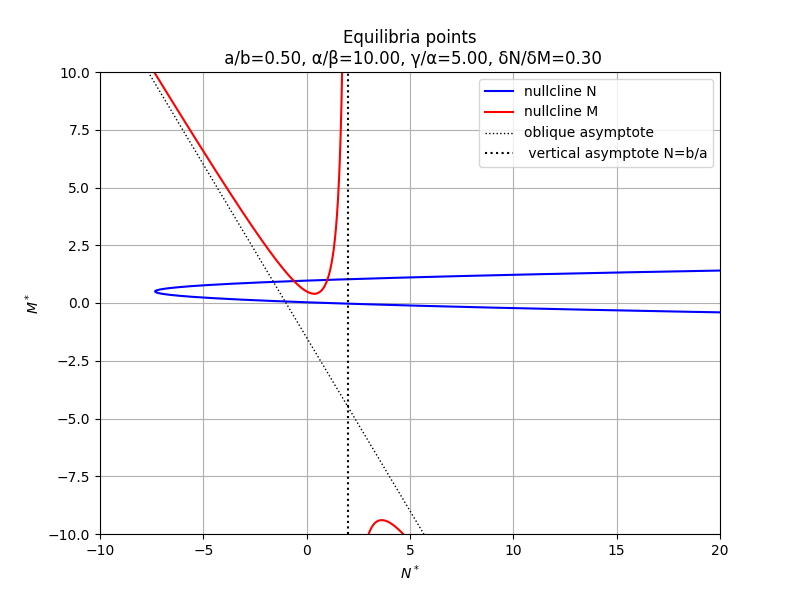
\includegraphics[width=0.45\textwidth]{equilibres_2.png}
%    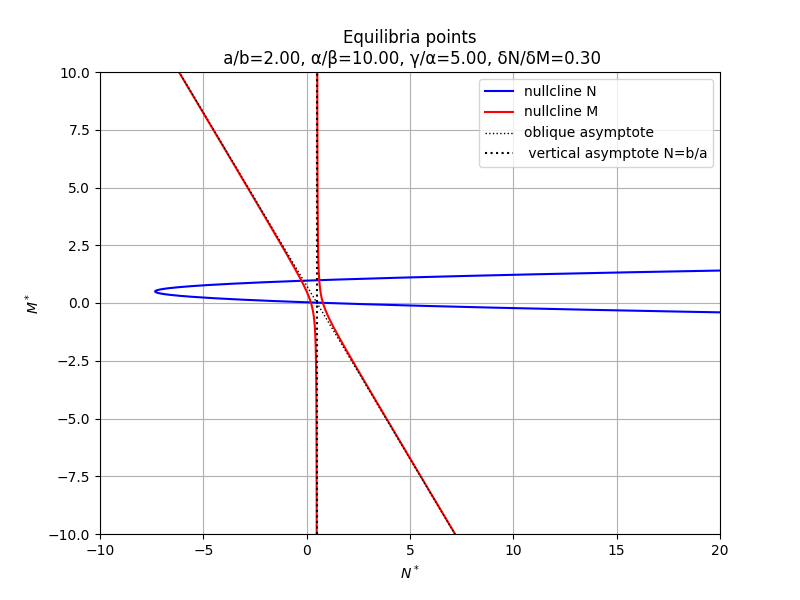
\includegraphics[width=0.45\textwidth]{equilibres_3.png}\\
%    \caption{equilibria in the $(N^*, M^*)$ plane, left $a < b$, right $a > b$.}
%    \label{fig:intersections}
%\end{figure}
\subsubsection{Equilibria points with $S^* \neq 0$.}
We express $N^*$ in terms of $T^*$ from equation \eqref{eq:equilibrium_S}:
\begin{equation}
N^* = \frac{b}{a} T^*
\label{eq:N_in_terms_of_T}
\end{equation}
Substituting this expression for $N^*$ into equation \eqref{eq:equilibrium_N}, we obtain:
\begin{equation}
S^* = \frac{\delta_N}{\alpha} \left(\frac{b}{a} T^* - 1\right)
\label{eq:S_in_terms_of_T}
\end{equation}
Since we are now looking for equilibria points with $S^* \neq 0$, \eqref{eq:equilibrium_M} and \eqref{eq:equilibrium_T} imply both $M^* \neq 1$ and $T^* \neq 1$.
 %Thus, we can express $M^*$ in terms of $S^*$ from equation \eqref{eq:equilibrium_M}: 
From equation \eqref{eq:equilibrium_M} and equation \eqref{eq:equilibrium_T}, 
we derive  $\delta_M M^* = \frac{\beta S^*}{M^* - 1}$ and $\delta_M M^* = \frac{\gamma S^* T^*}{1 - T^*}$.
Equating these two expressions for $\delta_M M^*$, we obtain:
\[\frac{\beta S^*}{M^* - 1} = \frac{\gamma S^* T^*}{1 - T^*}
\]
Assuming $S^* \neq 0$, we can simplify this equation to:
\[\frac{\beta}{M^* - 1} = \frac{\gamma T^*}{1 - T^*}
\]
From this, we can express $M^*$ in terms of $T^*$:
\begin{equation}
M^* = 1 + \frac{\beta (1 - T^*)}{\gamma T^*} = 1 - \frac{\beta}{\gamma} + \frac{\beta}{\gamma T^*}
\label{eq:M_in_terms_of_T}
\end{equation}  

Substituting the expression for $M^*$  and $S^*$ into the last equation \eqref{eq:equilibrium_T}, we obtain 
\begin{equation}
  -\gamma \frac{\delta_N}{\alpha} \left(\frac{b}{a} T^* - 1\right) T^* + \delta_M \left(1 - \frac{\beta}{\gamma} + \frac{\beta}{\gamma T^*}\right) (1 - T^*) = 0      
\end{equation}
Since $T^* \neq 0$, we can multiply this equation by $T^*$ and rearrange the terms to obtain a cubic equation for $T^*$:
\begin{equation}
\frac{\gamma}{\alpha} \frac{\delta_N}{\delta_M} \frac{b}{a} (T^*)^3 + \left( 1-   \frac{\gamma}{\alpha} \frac{\delta_N}{\delta_M}  - \frac{\beta}{\gamma}\right) (T^*)^2 + \left( 2\frac{\beta}{\gamma} -1 \right) T^* - \frac{\beta}{\gamma} = 0
\end{equation}
Rewriting this equation in the standard unitary form $(T^*)^3 + p (T^*)^2 + q T^* + r = 0$, we have:
\begin{equation}
\left(T^*\right)^3 + \frac{\alpha}{\gamma} \frac{\delta_M}{\delta_N} \frac{a}{b} \left(1- \frac{\beta}{\gamma} - \frac{\gamma}{\alpha} \frac{\delta_N}{\delta_M}\right) (T^*)^2 + \frac{\alpha}{\gamma} \frac{\delta_M}{\delta_N} \frac{a}{b} \left(2\frac{\beta}{\gamma} -1 \right) T^* - \frac{\alpha}{\gamma} \frac{\delta_M}{\delta_N} \frac{a}{b} \frac{\beta}{\gamma} = 0
\end{equation}
Notice that we need only 3 \emph{non dimensional} parameters $a/b$, $\beta/\gamma$, $\displaystyle{\frac{\gamma \delta_N}{\alpha \delta_M}}$ instead of the 7 original parameters.
%\begin{rem}
 %   The fact that only 3 non dimensional parameters determine the number of equilibria points with $S^* \neq 0$ suggests that it might be possible to reduce the original system \eqref{eq:system} to a simpler system depending only on these 3 parameters. 
  %  Although the equilibrium points depend indeed on 3 parameters only, the dynamical behavior could be more complex. Anyway it is not obvious to design the synthetic variables which could capture this complexity. They might not be easily expressible in terms of the original variables. This could be an interesting direction for further research.
%\end{rem}
In the following, we denote the 3 \emph{non dimensional} parameters as $A=a/b$, $B=\beta/\gamma$, and $C=\displaystyle{\frac{\gamma \,\delta_N}{\alpha\,\delta_M}}$.
\begin{rem}
The parameters $A$, $B$, and $C$ have the following biological interpretations:
\begin{itemize}
    \item $A = a/b$. This parameter represents the ratio of the inflammatory effect of the neutrophils w.r.t. the anti-inflammatory effect of the macrophages.
    \item $B = \beta/\gamma$. This parameter represents the ratio of the increasing rate of the Momac to the decreasing rate of the macrophage.
    \item $C = \frac{\gamma \,\delta_N}{\alpha\,\delta_M} = \left[\frac{\gamma}{\delta_M} : \frac{\alpha}{\delta_N}\right]$. This parameter represents the ratio of the macrophages vs the neutrophiles effects in the disease progression.
\end{itemize}   
\end{rem}
Using these parameters, the cubic equation in $T^*$ becomes:
\begin{equation} 
\left(T^*\right)^3 +  \frac{A}{C}  \left(1- B- C \right) (T^*)^2 + \frac{A}{C} \left(2 B -1 \right) T^* - \frac{A B}{C} = 0
\label{eq:cubic_T}
\end{equation} 
\begin{rem} Particular case $A = 1$.
There is an obvious solution in the particular case $A = a/b = 1$, namely $T^* = 1$. This solution corresponds to the inflammation free equilibrium point $S^* = 0, N^* = 1, M^* = 1, T^* = 1$.  
But this solution is not relevant for the case $S^* \neq 0$ that we are considering here.
Note further that if  $T^* = 1$  then  from Eq. \eqref{eq:cubic_T} we get
\[ 1 +  \frac{A}{C}  \left(1- B- C \right) + \frac{A}{C} \left(2 B -1 \right) - \frac{A B}{C} = 0
\]
which simplifies to $A = 1.$ Hence $T=1$ is a root of the cubic equation \eqref{eq:cubic_T} iff $A=1$.
Therefore we can factor the cubic polynomial as follows:
    \begin{equation}
    (T^* - 1) \left( (T^*)^2 - \frac{1}{C} (B - 1) T^* + \frac{B}{C} \right) = 0
    \label{eq:factored_cubic}
    \end{equation}
    \begin{itemize}
        \item If $B \leq 1$, then the coefficients of the quadratic factor are positive, hence there are no other positive roots.
        \item If $B > 1$, the quadratic factor has  either two positive roots (if the discriminant is positive) or no real roots (if the discriminant is negative).
    The quadratic factor has discriminant 
    $\Delta = \frac{(B-1)^2 - 4 B C }{C^2}$.
    Thus, we have:
    \begin{itemize}
        \item If $\Delta > 0$, there are two distinct real roots given by:
        \[
        T^* = \frac{\frac{(B- 1)}{C}  \pm \sqrt{\Delta}}{2}
        \]
        \item If $\Delta = 0$, there is one (double) positive root given by:
        \[
        T^*  = \frac{B - 1}{2 C}
        \]
        \item If $\Delta < 0$, there are no real roots.
    \end{itemize}
    \end{itemize}
\end{rem}
The sign of the discriminant of the quadratic factor depends on the parameters $B$ and $C$:  
$\Delta > 0$ iff $\frac{(B-1)^2}{4B} > C$.
Let us plot the curve $\frac{(B-1)^2}{4B}$ in the $(B,C)$ plane (see fig.\ref{fig:BC_plane}).    
\begin{figure}
    \centering
    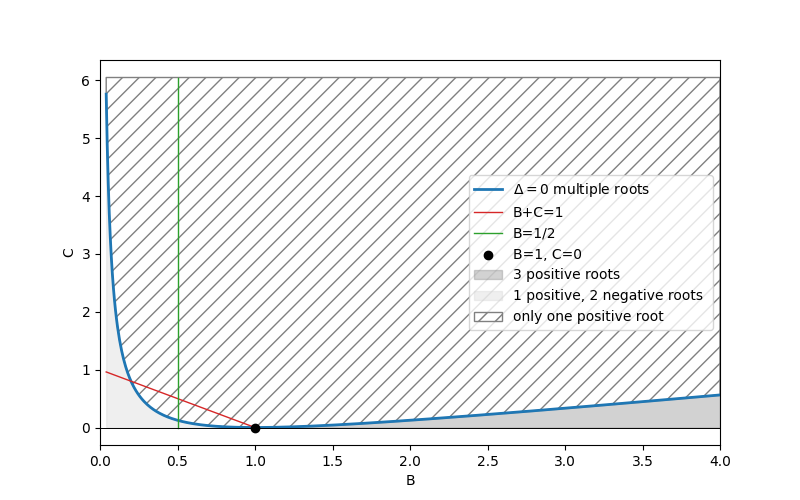
\includegraphics[height=5cm, width=0.6\textwidth]{discriminant_curve.png}
    \caption{ $A=1$, number of roots.}
    \label{fig:BC_plane}        
\end{figure}    
Looking  at  figure \ref{fig:BC_plane}, 
we see that the typical situation is when $\Delta < 0$, hence there are no other positive roots apart from $T^* = 1$.
But for a careful choice of parameters $B$ and $C$, we can indeed have three equilibria, see fig.\ref{fig:roots_A=1}. 
\begin{figure}
\centering
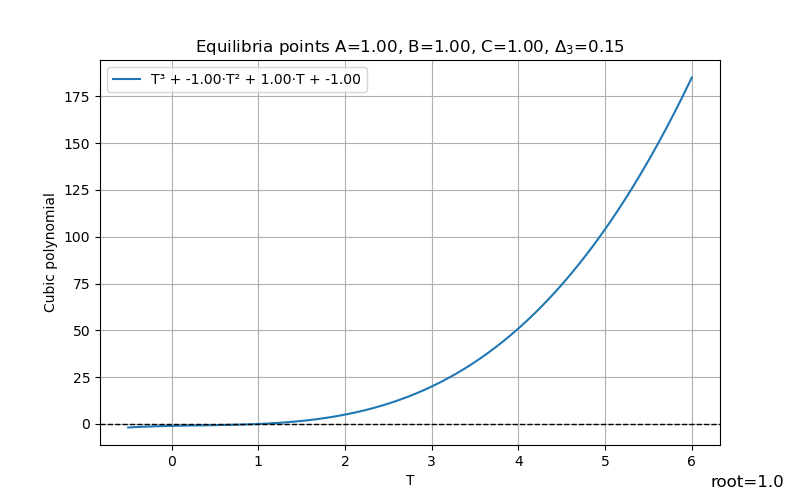
\includegraphics[height=4cm]{onepositive_A=1.png}
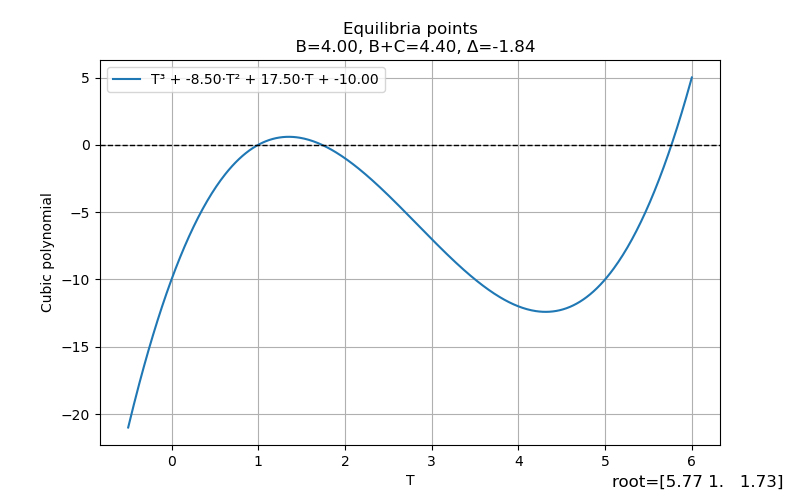
\includegraphics[height=4cm]{three_roots_A=1.png}
\caption{$A=1$, Left 1 positive root,\quad Right  3 positive roots}
\label{fig:roots_A=1}
\end{figure} 
\par\noindent Returning to the general case $A \neq 1$, we analyze the number of positive roots of the cubic equation \eqref{eq:cubic_T}.
From basic algebra, we can show that there are at most 3 such intersection points, hence at most 3 equilibria points with $S^* \neq 0$. 
We can be more precise because the biological feasibility imposes the roots to be real nonnegative numbers.
Since $\frac{AB}{C} > 0$,  there is at least one positive root. 
But we can be more precise using 
\emph{Descartes' rule of signs}. It states that the number of positive real roots of a polynomial (counting multiplicities) is equal to the number of sign changes between consecutive nonzero coefficients, or less than that by an even number. 
In our case, the coefficients of the cubic polynomial in \eqref{eq:cubic_T} are:
\[1, \quad \frac{A}{C} \left(1- B- C \right), \quad \frac{A}{C} \left(2 B -1 \right), \quad - \frac{A B}{C}   \]  
So the number of sign changes depends on the signs of the second and third coefficients.
We have the following cases:
\begin{itemize}
\item If $ B +C > 1$ and $B > 1/2$, then there are 3 sign changes and the cubic has one or three positive roots, which can collapse according to their multiplicities.
\item If $B +C  < 1$ and $B > 1/2 $, then there is one sign change and the cubic has only one positive roots.
\item If $B +C  < 1$ and $B < 1/2$, then there is one sign changes and the cubic has only one positive root.
\item If $B +C  > 1$ and $B < 1/2$, then there is one sign change and the cubic has only one positive root.
\end{itemize}
\bigskip
We can plot some typical cases in the following figure (see figure \ref{fig:cubics}).
\begin{figure}[!htbp]
    \centering
    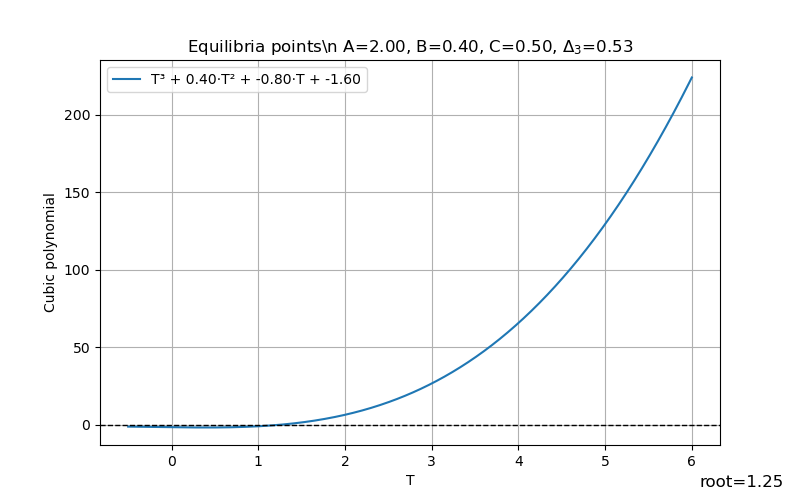
\includegraphics[width=0.45\textwidth, height=5cm]{cubic_1.png}
    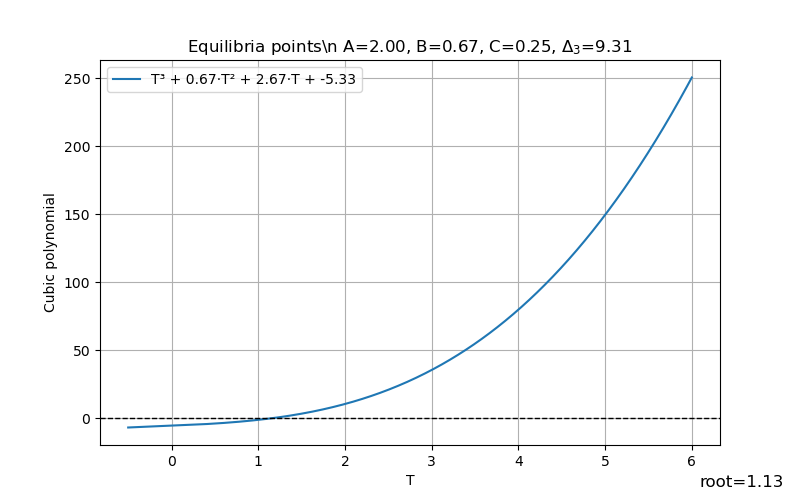
\includegraphics[width=0.45\textwidth, height=5cm]{cubic_2.png}\\
    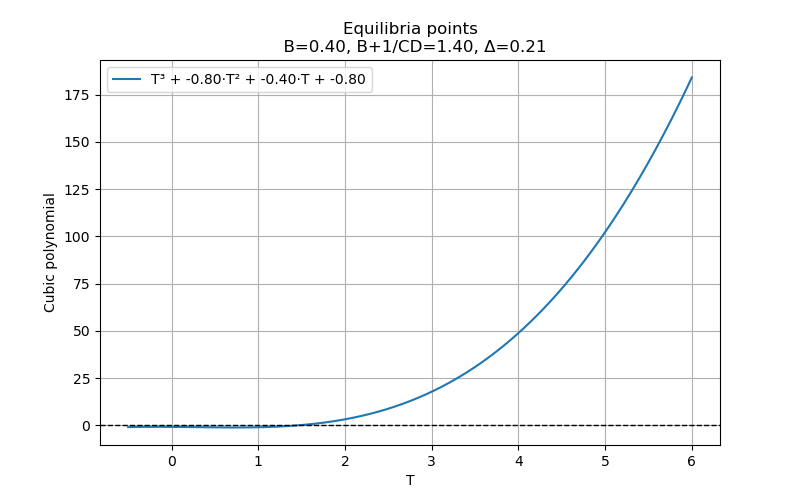
\includegraphics[width=0.45\textwidth, height=5cm]{cubic_3.png}
    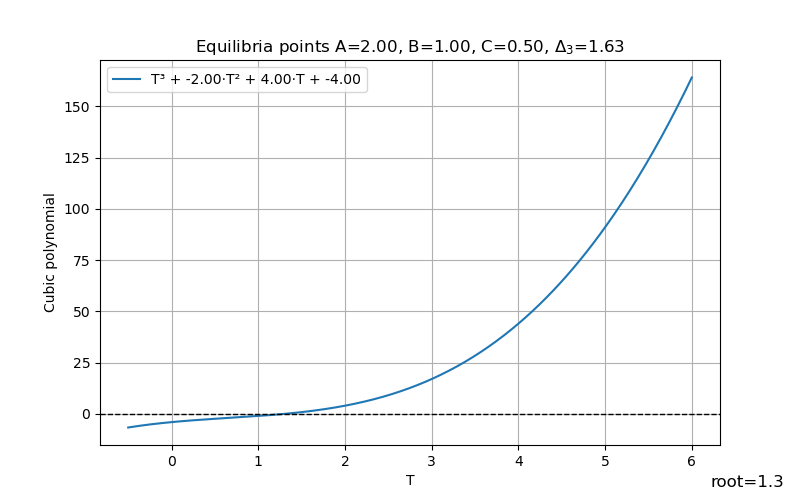
\includegraphics[width=0.45\textwidth, height=5cm]{cubic_4.png}\\
    \caption{Cubic equation in $T^*$, left $B<1/2$, right $B>1/2$.}
    \label{fig:cubics}
\end{figure}

\par\noindent We can use Cardano's method to find the roots of the cubic equation \eqref{eq:cubic_T}. We rewrite it in the standard form:
\[ T^3 + p T^2 + q T + r = 0
\]
where
\[ p = \frac{A}{C} \left(1- B- C \right), \quad
q = \frac{A}{C} \left(2 B -1 \right), \quad
r = -\frac{A B}{C}
\]
We perform the change of variable $T = x - p/3$ to eliminate the quadratic term and obtain the depressed cubic equation:
\[
x^3 + \mathcal{A} x + \mathcal{B} = 0
\]
where
\[
\mathcal{A} = q - \frac{p^2}{3}, \quad \mathcal{B} = \frac{2 p^3}{27} - \frac{p q}{3} + r
\]
The discriminant of this equation is given by:
\[
\Delta_3 = \left(\frac{\mathcal{B}}{2}\right)^2 + \left(\frac{\mathcal{A}}{3}\right)^3
\]

The nature of the roots depends on the sign of the discriminant $\Delta_3$:
\begin{itemize}
\item If $\Delta_3 > 0$, there is one real root and two complex conjugate roots.
\item If $\Delta_3 = 0$, all roots are real and at least two are equal.
\item If $\Delta_3 < 0$, all roots are real and unequal.
\end{itemize}
Hence we can characterize the case when we have three distinct real roots by the condition $\Delta_3 < 0$, which is equivalent to:
\[ \left(\frac{\mathcal{A}}{3}\right)^3 < - \left(\frac{\mathcal{B}}{2}\right)^2.
\]
The parameters $\mathcal{A}$ and $\mathcal{B}$ can be rewritten in terms of the original parameters  using computer algebra as follows:
%%%% TO DO: compute again with sympy
\[
\mathcal{A}=\frac{A}{ 3 C^2} \Big(-A (B + C - 1)^2 + 3 C(2B - 1)\Big)
\]
\[
\mathcal{B}= \frac{A} {27 C^3} \Big(-2A^2 (B + C - 1)^3 + 9 A C (2 B - 1)(B + C - 1) - 27 B C^2\Big)
\]
The discriminant $\Delta_3$ can be rewritten in terms of the original parameters as follows:
\[
\Delta_3 = \frac{A^2} {108 C^4} \Bigg(A^2 (4BC-1) (B + C - 1)^2 - 2AC (2B-1)(B^2-9BC-B-2) + 27 B^2 C^2\Bigg)
\]
\par\noindent



The real roots can be found using Cardano's formulas. 
If $\Delta_3 > 0$, the real root is given by:
\[
x^* = \sqrt[3]{-\frac{\mathcal{B}}{2} + \sqrt{\Delta_3}} + \sqrt[3]{-\frac{\mathcal{B}}{2} - \sqrt{\Delta_3}}
\]
If $\Delta_3 < 0$, the three real roots are given by:
\[
x_k^* = 2 \sqrt{-\frac{\mathcal{A}}{3}} \cos\left(\frac{1}{3} \arccos\left(\frac{3 \mathcal{B}}{2 \mathcal{A}} \sqrt{-\frac{3}{\mathcal{A}}}\right) + \frac{2 k \pi}{3}\right), \quad k = 0, 1, 2
\]
If $\Delta_3 = 0$, the real roots are given by:
\[x_1^* = 2 \sqrt[3]{-\frac{\mathcal{B}}{2}}, \quad x_2^* = x_3^* =  \sqrt[3]{\frac{\mathcal{B}}{2}}
\]
\par\noindent
Here we plot a case with three distinct positive roots (see figure \ref{fig:three_roots}).
Namely we take $A = 1.1$, $B = 5$ and $C = \frac{2}{3}$.
\begin{figure}[htbp]
    \centering
    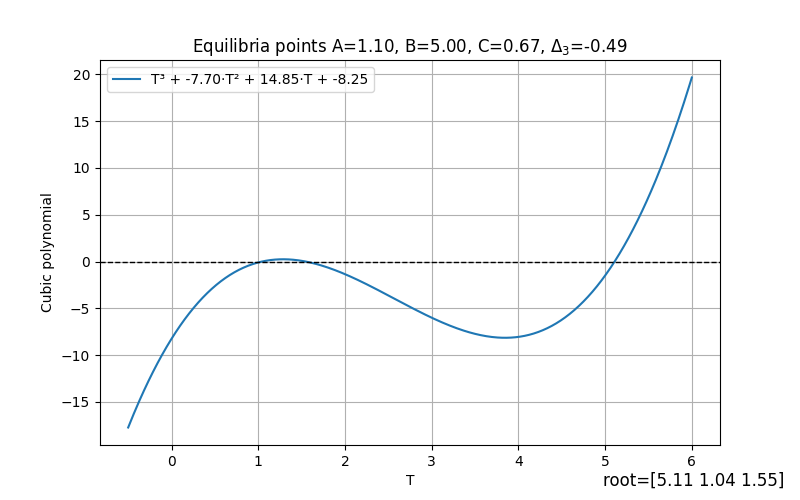
\includegraphics[width=0.6\textwidth]{three_roots.png}
    \caption{Cubic equation with three distinct real roots.}
    \label{fig:three_roots}
\end{figure}
% \begin{rem}
%     there is an interesting phenomenon of potential \emph{bifurcation} when the parameters vary and the number of equilibria points changes. This is a topic for further study.
% In particular, when the equilibrium point with $S^* \neq 0$  when $S^* \ll 1$ is close to the disease-free equilibrium point $S^* = 0, N^* = 1, M^* = 1, T^* = 1$, we can perform a local stability analysis using perturbation methods.
% We should analyze this with the tool of catastrophe theory.
% \end{rem}
\par\noindent 
Finally, we can recover the roots $T^*$ of the original cubic equation 
using the relation $T^* = x^* - p/3$.
\bigskip\\
We have to make sure that the nonegative roots $T^*$ found are biologically feasible, i.e. that they lead to nonnegative values of $S^*$, $N^*$, and $M^*$.
For instance in the case $A=1.1$, $B=5$, $C=2/3$ plotted in figure \ref{fig:three_roots}, we have three distinct positive roots of the cubic equation \eqref{eq:cubic_T},
but none satisfying the biological feasibility conditions.\smallskip\\
From equations \eqref{eq:N_in_terms_of_T}, \eqref{eq:S_in_terms_of_T}, and \eqref{eq:M_in_terms_of_T}, we have: 
\[N^* = \frac{b}{a} T^*, \quad S^* = \frac{\delta_N}{\alpha} \left(\frac{b}{a} T^* - 1\right), \quad M^* = 1 - \frac{\beta}{\gamma} + \frac{\beta}{\gamma T^*}
\]
Thus, the conditions for biological feasibility are:
\begin{itemize}
\item $S^* \geq 0$ iff $T^* \geq \frac{a}{b} = A$  
\item $N^* \geq 0$  iff $T^* \geq 0$ (always true since we consider only positive roots)
\item $M^* \geq 0$  iff $T^* \leq \frac{\beta}{\beta - \gamma}= \frac{B}{B-1}= 1 + \frac{1}{B-1}$ if $B= \frac{\beta}{\gamma} > 1$; always true if $B \leq 1$.
\end{itemize}
So the biological feasibility conditions can be summarized as follows:
\begin{eqnarray}
T^* &\geq& A \label{feas_T1} \\
T^* &\leq& 1 + \frac{1}{B-1} \quad \text{if } B > 1 \label{feas_T2}
\end{eqnarray}
Let us consider again the particular case $A = a/b = 1$, if $B \leq 1$  there is only one equilibrium, the disease-free $(S^*, N^*, M^*, T^*) = (0, 1, 1, 1)$ otherwise if $B>1$ the feasibility conditions \eqref{feas_T1}-\eqref{feas_T2} reduce to:
\begin{equation}
1 \leq T^* \leq 1 + \frac{1}{B-1}.
\end{equation}
 We can check easily that only the disease-free root $T^* = 1$ satisfies this condition, while the other two roots are outside this interval (see figure \ref{fig:roots_A=1}).
 Indeed if $\Delta \geq 0$, we have $C \leq \frac{(B-1)^2}{4B}$, 
 hence $\frac{B-1}{2C} \geq \frac{B-1}{2 \frac{(B-1)^2}{4B}} = \frac{2B}{B-1} \geq 2  $ so  the root $T^* = \frac{B-1 + \sqrt{\Delta}}{2C} \geq 2  $ is not feasible.
 Moreover, the other root $T^* = \frac{B-1 - \sqrt{\Delta}}{2C} \leq \frac{B-1}{2C}.$
 In order to be feasible, this root should satisfy $\frac{B-1 - \sqrt{\Delta}}{2C} \leq \frac{B}{B-1}$,
which implies  $C \geq \frac{(B-1)^2}{2B}$, contradicting the assumption $\Delta \geq 0$.
\bigskip\\
In the general case $A \neq 1$, the feasibility conditions \eqref{feas_T1}-\eqref{feas_T2} have to be checked for each positive root found. 
For $A>1$, we will show that none of the positive roots satisfy the feasibility conditions (see figure \ref{fig:three_roots}) whereas for $A<1$, there is always exactly one feasible root (in addition to the disease-free equilibrium) (see figure \ref{fig:feasible_region}).
To this aim, we consider four cases  depending on the signs of $A - 1$ and $B - 1$.
\begin{description}
\item[-] Case $A > 1$ and $B \geq 1$.\\ 
Let us define $f(T^*)$ as the cubic polynomial in the left-hand side of equation \eqref{eq:cubic_T}. 
If $B>1$ we have
\begin{eqnarray*}
f(T^*)&=&{T^*}^3-\frac{A}{C}(B-1){T^*}^2-A{T^*}^2+\frac{A}{C}(B-1)T^*+\frac{A}{C}BT^*-\frac{AB}{C}\\\nonumber
&=&\frac{A}{C}(B-1)(T^*-\frac{B}{B-1})(1-T^*)+{T^*}^2(T^*-A)
\end{eqnarray*} 
So $f(T^*)>0$, for $T^* \in [A, \frac{B}{B-1}]$  if $B>1$.\\
If $B=1$ then $f(T^*)={T^*}^2(T^*-A)+\frac{A}{C}(T^*-1)>0$ for $T^*>A$.\\
Hence, thanks to \eqref{feas_T1} and \eqref{feas_T2}, there is no feasible root in this case.
\item[-] Case $A > 1$ and $B < 1$.
Since \begin{eqnarray*}
f(T^*)=\frac{A}{C}(B-1)(T^*-\frac{B}{B-1})(1-T^*)+{T^*}^2(T^*-A)&>&0
\end{eqnarray*}
for $T^* \geq A$ and $B<1$, there is no feasible root in this case either. 
\item[-] Case $A < 1$ and $B  \geq1$.\\
We compute $f(1)=1-A>0$ and $f(A)=(A-1)\frac{A}{C}(A(1-B)+B)<0$, so there is at least one feasible root in this case.\\
If $B>1$, computing the derivative $f'(T^*)$ we have:
\begin{eqnarray*}
f'(T^*) &=& \frac{A}{C}(B-1)\big[(\frac{B}{B-1}-T^*)+(1-T^*)\big]+2{T^*}(T^*-A)+{T^*}^2 >0
\end{eqnarray*}
for $T^* \in [A,1]$. So there is exactly one root in the interval $[A,1]$.
Since once again $f(T^*)=\frac{A}{C}(B-1)(T^*-\frac{B}{B-1})(1-T^*)+{T^*}^2(T^*-A)$ is positive for $T^* \in [1, \frac{B}{B-1}]$, there is exactly one feasible root in this case.\\
If $B=1$, we have $f(T^*)={T^*}^2(T^*-A)+\frac{A}{C}(T^*-1)>0$ for $T^*>1$ and $f'(T^*)={T^*}^2+2{T^*}({T^*}-A)+\frac{A}{C}>0$ for $T^* \in [A,1]$. 
So there is exactly one feasible root in this case too.
\item[-] Case $A < 1$ and $B < 1$.\\
Since $f(1)=1-A>0$ and $f(A)=(A-1)\frac{A}{C}(A(1-B)+B)<0$, there is at least one feasible root in this case too.
Let $\tilde{T}=T^*-A$ and $\tilde{f}(\tilde{T})=f(\tilde{T}+A)$. Then the equation $\tilde{f}(\tilde{T})=0$ is written as:
\begin{eqnarray*}
\tilde{T}^3 +\left(3A+\frac{A}{C}(1-B-C)\right)\tilde{T}^2&+&\left(3A^2+2\frac{A^2}{C}(1-B-C)+\frac{A}{C}(2B-1)\right)\tilde{T}\\
&+&\frac{A}{C}(A-1)\left(A(1-B)+B\right)\\
    =\tilde{T}^3+\left(2A+\frac{A}{C}(1-B)\right)\tilde{T}^2&+&\left(A^2+2\frac{A^2}{C}(1-B)+\frac{A}{C}(2B-1)\right)\tilde{T}\\
    &+&\frac{A}{C}(A-1)\left(A(1-B)+B\right)=0.
    \end{eqnarray*}
    Using {\sl Descartes' rule of signs} we can see that there is exactly one positive root $\tilde{T}$ 
    of the cubic equation $\tilde{f}(\tilde{T})=0$  as the coefficients of $\tilde{T}^3$ and $\tilde{T}^2$ are positive and the constant term is negative. 
    So there is exactly one feasible root $T^*\geq A$ in this case too.
\end{description}
\par\noindent Let us summarize. The feasible equilibria points of the system can be classified as follows:
\begin{itemize}
\item Disease-free equilibrium: $(S^*, N^*, M^*, T^*) = (0, 1, 1, 1)$.
\item Other equilibria with $S^* = 0$: 
$S^* = 0, N^* = 0, M^* = 0, T^* = R$, with arbitrary $R$;
 $S^* = 0, N^* = 0, M^* = 1, T^* = 1$;
 $S^* = 0, N^* = 1, M^* = 0, T^* = R$, with arbitrary $R$.
\item Feasible equilibria with $S^* \neq 0$: 
None when $A \geq 1$. We shall see in the numerical simulations that in this case the system quickly diverges away from the disease-free equilibrium, no matter how weak is the initial inflammation. This suggests that the system is in a chronic inflammatory state with $S^* \neq 0$.
When $A < 1$, there is only one biologically feasible equilibria with $S^* \neq 0$ (see proof and figure \ref{fig:feasible_region}). We shall see in the next section that this equilibrium is unstable, and the numerical simulations suggest that the system converges to the disease-free equilibrium, hence the inflammation is resolved.
\end{itemize} 
\begin{figure}[htbp]
    \centering
    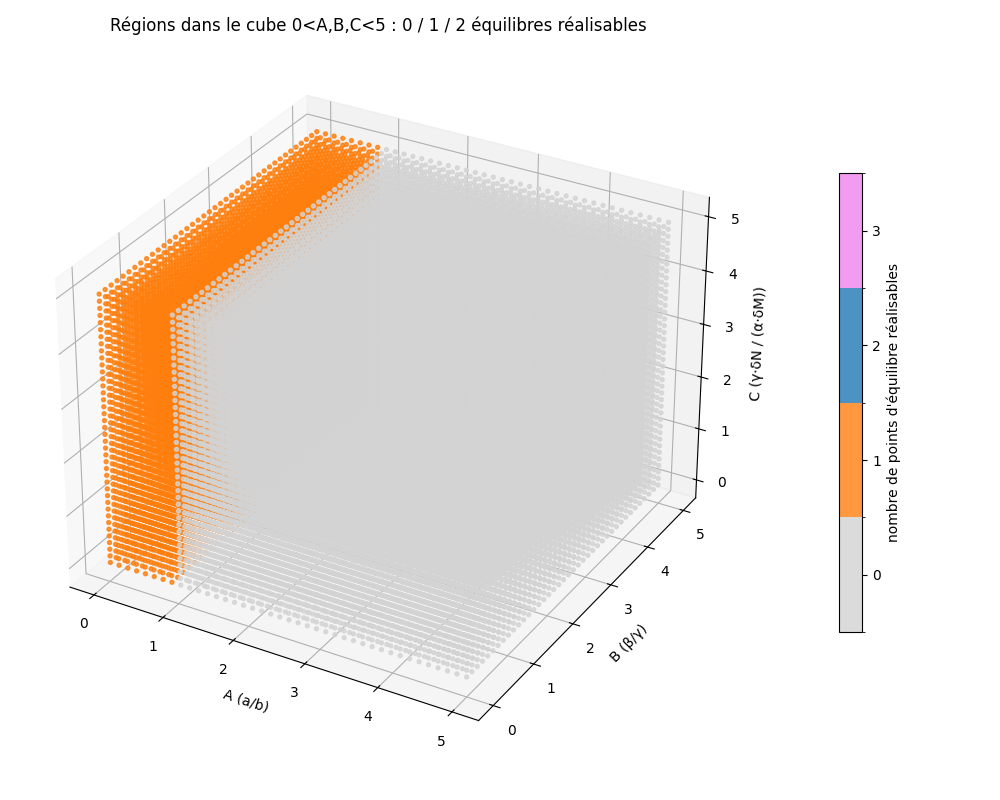
\includegraphics[width=0.6\textwidth]{feasibility_regions_3D.png}
    \caption{Feasible region in the $(A,B,C)$ space, when $S^* \neq 0$.}
    \label{fig:feasible_region}
\end{figure}      
\subsection{Stability analysis}
\emph{Linear stability analysis} of the equilibria point $ (S^*, N^*, M^*, T^*)$ is done by linearizing the system around this point.
The Jacobian matrix of the system is given by:
\[
J = \begin{pmatrix}
aN - bT & aS & 0 & -bS \\
\alpha N & \alpha S - \delta_N (2N-1) & 0 & 0 \\
\beta & 0 & -\delta_M (2M-1) & 0 \\
-\gamma T & 0 & \delta_M (1-T) & -\gamma S - \delta_M M
\end{pmatrix}
\]
According to the linear stability theory, the equilibrium point is (locally asymptotically) stable if all eigenvalues of the Jacobian matrix have negative real parts, and unstable if at least one eigenvalue has a positive real part. In what follows,
 we analyze the stability of the different equilibria points found in the previous section. By locally asymptotically stable, we mean that if the system is perturbed slightly from the equilibrium point, it will return to the equilibrium point as time goes to infinity. On the other hand, if the equilibrium point is unstable, a small perturbation will cause the system to move away from the equilibrium point.
\subsubsection{Stability of  inflammation free equilibria ($S^* =0$).}\label{sec:stab}
We analyze first the stability of the disease-free equilibrium point $(S^*, N^*, M^*, T^*) = (0, 1, 1, 1)$.
At this point, the Jacobian matrix simplifies to:
\[
J|_{(S^*, N^*, M^*, T^*) = (0, 1, 1, 1)} =
\begin{pmatrix}
a - b & 0 & 0 & 0 \\
\alpha & - \delta_N & 0 & 0 \\
\beta & 0 & -\delta_M & 0 \\
-\gamma & 0 & 0 & -\delta_M
\end{pmatrix}
\]
We notice immediately that the eigenvalues of this matrix are  $a-b$, $-\delta_N$ and $-\delta_M$.
 The last two are negative since $\delta_N, \delta_M > 0$. The remaining eigenvalue  is $a-b$. Thus the disease-free equilibrium is stable if $a < b$ and unstable if $a > b$. 
This means that if the inflammatory effect of Neutrophiles cells controlled by paramater $a$ is less than the curing effect of the  SL-TRM macrophages controlled by parameter $b$, the system will return to the disease-free state. Conversely, if $a > b$, the system may move away from this equilibrium, potentially leading to a chronic inflammatory state.
The particular case $a = b$ corresponds to a bifurcation point where the stability of the disease-free equilibrium changes. In this case, a more detailed analysis is needed to determine the behavior of the system near this point, which  involve higher-order terms in the Taylor expansion of the system around the equilibrium.
The numerical simulations, see section \ref{sec:numerical_simulations} suggest that for $a=b$ the system quickly diverges from the disease-free equilibrium, and indeed this equilibrium is unstable in this case as we prove below using the center manifold theory.
\par For $a=b$ the disease-free equilibrium is a non-hyperbolic equilibrium with eigenvalues $0$, $-\delta_N$, $-\delta_M$ and $-\delta_M$. 
The stability of this equilibrium can be analyzed using center manifold theory. We prove here that the center manifold is repulsive for $S^* \geq 0$, hence the equilibrium is unstable.\\
In this case there is one center direction and three stable directions. We define new variables $x=S$, $y=N-1$, $z=M-1$, and $w=T-1$ to shift the equilibrium point to the origin. The system can be rewritten as:
\begin{eqnarray*}
\dot{x} &=&  ax (y - w) \\
\dot{y} &=& (y+1)(\alpha x - \delta_N y ) \\
\dot{z} &=& \beta x - \delta_M z (z+1)\\
\dot{w} &=& -\gamma x(w + 1) - \delta_M w (z+ 1)
\end{eqnarray*} 
The linear part of the system is given by:
\begin{eqnarray*}
\dot{x} &=& 0 \\
\dot{y} &=&\alpha x - \delta_N y \\
\dot{z} &=&\beta x - \delta_M z \\
\dot{w} &=&-\gamma x - \delta_M w
\end{eqnarray*}
where the center direction is given by the variable $x$ and the stable directions are given by the variables $y$, $z$, and $w$.
The center manifold can be expressed as a graph of the form $h(x) = (h_1(x), h_2(x), h_3(x))$ where $h_i(0) = 0$ for $i=1,2,3$.
We can compute the Taylor expansion of $h$ and find that the first nonzero term is given by $h_1(x) = \frac{\alpha}{\delta_N} x + o(x)$, $h_2(x) = \frac{\beta}{\delta_M} x + o(x)$, and $h_3(x) = -\frac{\gamma}{\delta_M} x + o(x)$.
The dynamics on the center manifold is given by: 
\begin{eqnarray*}
\dot{x} &=& ax^2(\frac{\alpha}{\delta_N}+ \frac{\gamma}{\delta_M}) + o(x^2)
\end{eqnarray*}
Since $\frac{\alpha}{\delta_N}+ \frac{\gamma}{\delta_M} > 0$, the center manifold is repulsive for $x \geq 0$, hence the equilibrium is unstable.

The stability of other equilibria points can be analyzed similarly by evaluating the Jacobian matrix at those points and determining the eigenvalues.
\par\noindent For $S^* = 0, N^* = 0, M^* = 0, T^* = R$, with arbitrary $R$, the Jacobian matrix becomes:
\[
J|_{(S^*, N^*, M^*, T^*) = (0, 0, 0, R)} =
\begin{pmatrix}
- b R & 0 & 0 & 0 \\
0 & \delta_N & 0 & 0 \\
\beta & 0 & \delta_M & 0 \\
-\gamma R & 0 & \delta_M (1 - R) & 0
\end{pmatrix}
\]
The eigenvalues of this matrix are $-b R$, $\delta_N$, $\delta_M$, and $0$. Since $\delta_N$ and $\delta_M$ are positive, this equilibrium point is unstable. Even if the immune signal will decrease exponentially fast, the populations of neutrophiles and Momac will grow out of bound. This unstable equilibrium where the inflammation is zero as well as the population of neutrophiles and Momac is highly unlikely to be observed in practice.
\par\noindent For $S^* = 0, N^* = 0, M^* = 1, T^* = 1$, the Jacobian matrix is:
\[
J|_{(S^*, N^*, M^*, T^*) = (0, 0, 1, 1)} =
\begin{pmatrix}
-b & 0 & 0 & 0 \\
0 & \delta_N & 0 & 0 \\
\beta & 0 & -\delta_M & 0 \\
-\gamma & 0 & 0 & -\delta_M
\end{pmatrix}
\]
The eigenvalues of this matrix are $-b$, $\delta_N$, $-\delta_M$, and $-\gamma$. Since there is a positive eigenvalue , this equilibrium point is unstable. Neutrophiles can grow out of bound. This equilibrium will not be observed in practice neither.
\par\noindent For $S^* = 0, N^* = 1, M^* = 0, T^* = R$, with arbitrary $R$, the Jacobian matrix is
\[
J|_{(S^*, N^*, M^*, T^*) = (0, 1, 0, R)} =
\begin{pmatrix}
a - b R & 0 & 0 & 0 \\
\alpha & -\delta_N & 0 & 0 \\
\beta & 0 & \delta_M & 0 \\
-\gamma R & 0 & \delta_M (1 - R) & 0
\end{pmatrix}
\]
There is a positive eigenvalue $\delta_M$, hence this equilibrium point is unstable. Momac can grow out of bound. This equilibrium will not be observed in practice neither.
\subsubsection{Stability of equilibrium with $S^*\neq 0$.}
The stability of the equilibria with $S^* \neq 0$ can be analyzed similarly by evaluating the Jacobian matrix at those points and determining the eigenvalues.
Taking into account the equilibrium equations \eqref{eq:equilibrium_S}, \eqref{eq:equilibrium_N}, and \eqref{eq:equilibrium_T}, the Jacobian matrix at $(S^*, N^*, M^*, T^*)$ is:

\[
J = \begin{pmatrix}
0 & aS & 0 & -bS \\
\alpha N &  - \delta_N (N) & 0 & 0 \\
\beta & 0 & -\delta_M (2M-1) & 0 \\
-\gamma T & 0 & \delta_M (1-T) & - \delta_M\frac{M}{T} 
\end{pmatrix}
\]
The eigenvalues of this matrix can be found by solving the characteristic polynomial $\det(J - \lambda I) = 0$. A straightforward computation shows that the characteristic polynomial is given by:
\begin{eqnarray*}
&P(\lambda) = \lambda^4 + \Big(\delta_N N + \delta_M (2M-1) + \delta_M \frac{M}{T}\Big) \lambda^3 \\
&+ \Big(\delta_N N \delta_M(2M-1 + \frac{M}{T}) + {\delta_M}^2 (2M-1)\frac{M}{T} -a S \alpha N - b S \beta \gamma \Big) \lambda^2 \\
&+ \Big(- a S \alpha N \delta_M (2M-1+\frac{M}{T})  - b S\gamma T\delta_N N + \delta_N N {\delta_M}^2(2M-1)\frac{M}{T}- b{\delta_M}^2 M^2(1-T)\Big) \lambda \\
&- a S \alpha N {\delta_M}^2 (2M-1) \frac{M}{T} - b \delta_N N {\delta_M}^2 M^2 (1-T)
\end{eqnarray*}
Due to the Descartes' rule of signs, we claim that the polynomial $P(\lambda)$ has one positive root (hence the equilibrium is unstable). Indeed, the coefficients of $P(\lambda)$ are positive for the terms in 
$\lambda^4$ and $\lambda^3$, whereas the constant term is negative. To prove that there is only one change of sign and hence one positive root, we have to check that if the coefficient of $\lambda$ is positive then the coefficient of 
$\lambda^2$ is positive too. 

\noindent
If the coefficient of $\lambda$ is positive we have the following inequality:
\[
 a S \alpha N \delta_M (2M-1+\frac{M}{T})+ b{\delta_M}^2 M^2(1-T)+ b S\gamma T\delta_N N < \delta_N N {\delta_M}^2(2M-1)\frac{M}{T}
\]
Thanks to the positivity of all terms, we can deduce the following inequalities:
\begin{equation}
 a S \alpha N \delta_M (2M-1+\frac{M}{T}) < \delta_N N {\delta_M}^2(2M-1)\frac{M}{T},
\label{ineq1}
\end{equation}
and
\begin{equation}
 b S\gamma T < {\delta_M}^2(2M-1)\frac{M}{T}.
\label{ineq2}
\end{equation}
Inequality \eqref{ineq1} implies that 
\begin{equation}\label{ineq3}
a S \alpha N < a S \alpha N\left(\frac{{\delta_M}^2 {(2M-1+\frac{M}{T}) }^2}{{\delta_M}^2(2M-1)\frac{M}{T}}\right)<\delta_N N \delta_M (2M-1+\frac{M}{T}).
\end{equation}
Due to \eqref{ineq2} and \eqref{ineq3}, the coefficient of $\lambda^2$ is positive.
\par\noindent
We proved that biologically feasible equilibrium with $S^* \neq 0$ only exists if $A<1$ and is unstable.
For $A\geq 1$ the only biologically feasible equilibrium is the disease-free equilibrium which is unstable, as we have seen.

\subsection{Bifurcation diagram}
We perform a bifurcation analysis with respect to the \emph{non dimensional} parameters $A=a/b$. We restict to the biologically relevant feasible equilibria.
From the stability analysis above, we see that we  have only one  bifurcation at  $A=1$: for $A<1$ there are two biologically feasible equilibria, one  inflammatory one with $S^* \neq 0$ which is unstable and the disease-free equilibrium which  is stable; 
for $A\geq 1$ the disease-free equilibrium is unstable and there is no other biologically feasible equilibrium.
The number and stability of equilibria change as the parameter $A$ crosses the critical value $A=1$, indicating bifurcation points in the system's dynamics.   
We can plot the bifurcation diagram in the $(A,S^*)$ plane (see figure \ref{fig:bifurcation}).
\begin{figure}
 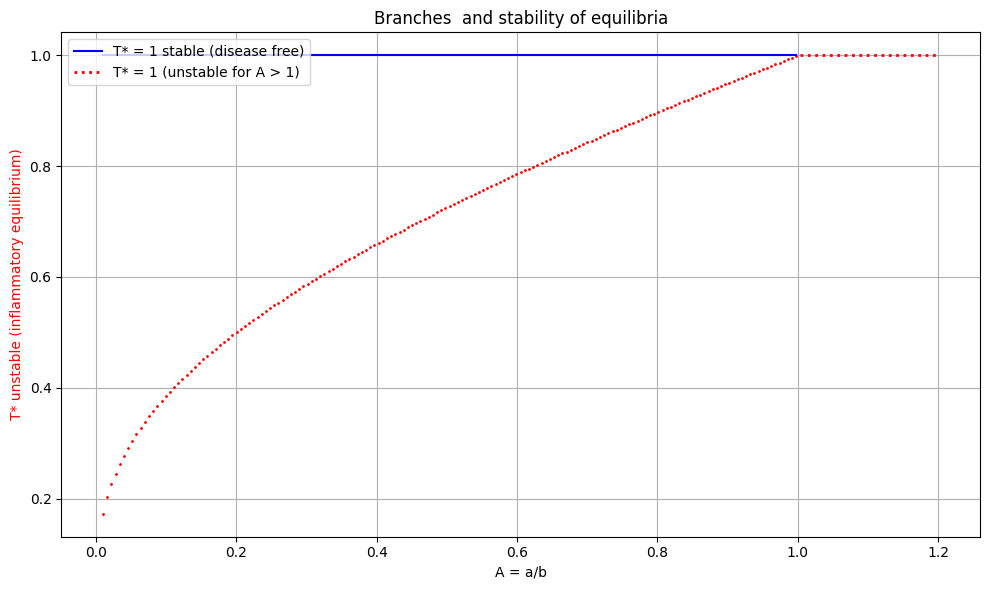
\includegraphics[scale=0.5]{bifurcation.png}      
 \caption{Bifurcation diagram in the $(A,T^*)$ plane.}
 \label{fig:bifurcation}
\end{figure}
%\par\noindent
%\bigskip\\
%\begin{center}
%\begin{tikzpicture}
%\node[draw=gray!60, fill=gray!5, rounded corners, inner sep=8pt] (box) {
%    \begin{minipage}{0.86\textwidth}
%        \centering
%        {\Large\bfseries\color{blue}To Do List}\\[6pt]
%        \begin{itemize}
            %\item[$\blacksquare$] \textcolor{black}{Is there a way to reduce the system introducing new nonlinear variables, depending only on the 3  adimensional parameters?}
            %\item[$\blacksquare$] \textcolor{black}{Recompute equilibria and simplify algebra}
            %\item[$\blacksquare$] \textcolor{black}{Write Python code to compute equilibria numerically}
            %\item[$\blacksquare$] {\textcolor{red}{perform stability analysis of non homeostasic equilibria (chronic inflammation)}}
            %\item[$\blacksquare$] \textcolor{red}{Perform bifurcation analysis and plot results}
            %\item[$\blacksquare$] \textcolor{blue}{compute attracting sets for A=1/ when there is a zero eigenvalue (center manifold theory)}
            %\item[$\blacksquare$] \textcolor{blue}{is there hysteresis phenomenon? compute domain of persistence/ disease-free attraction basins in the (S,A) plane as in Torres et al. 2024}
            %\item[$\blacksquare$] \textcolor{blue}{Plot 4d phase space trajectories (projections)}
            %\item[$\blacksquare$] \textcolor{blue}{Plot 2d phase space trajectories (Momac, Monocytes) or (neutrophiles, monocytes)(projections)}
            %\item[$\blacksquare$] \textcolor{blue}{Run numerical simulations with realistic rates}
            %\item[$\blacksquare$] \textcolor{blue}{perform sensitivity analysis of parameters}
            %\item[$\blacksquare$] \textcolor{blue}{calibrate results with immunology collaborators}
            %\item[$\blacksquare$] \textcolor{red}{use optimal control theory to model treatments (corticosteroids, anti TNF alpha, ethanecerp, inhibitor of neutrophiles degranulation,...)}
        %\end{itemize}
    %\end{minipage}
%\end{tikzpicture}
%\end{center}
\section{Numerical simulations}\label{sec:numerical_simulations}
Here we reproduce some typical simulations of the model using the following parameters:
$\alpha=1, \beta=1, \gamma=1,
       \delta_N=1, \delta_M=1, a=0.35,\; b=1$,  duration=20 days and initial conditions $S(0)=1, N(0)=1, M(0)=1, T(0)=1$.
\begin{figure}[htbp]
    \centering
    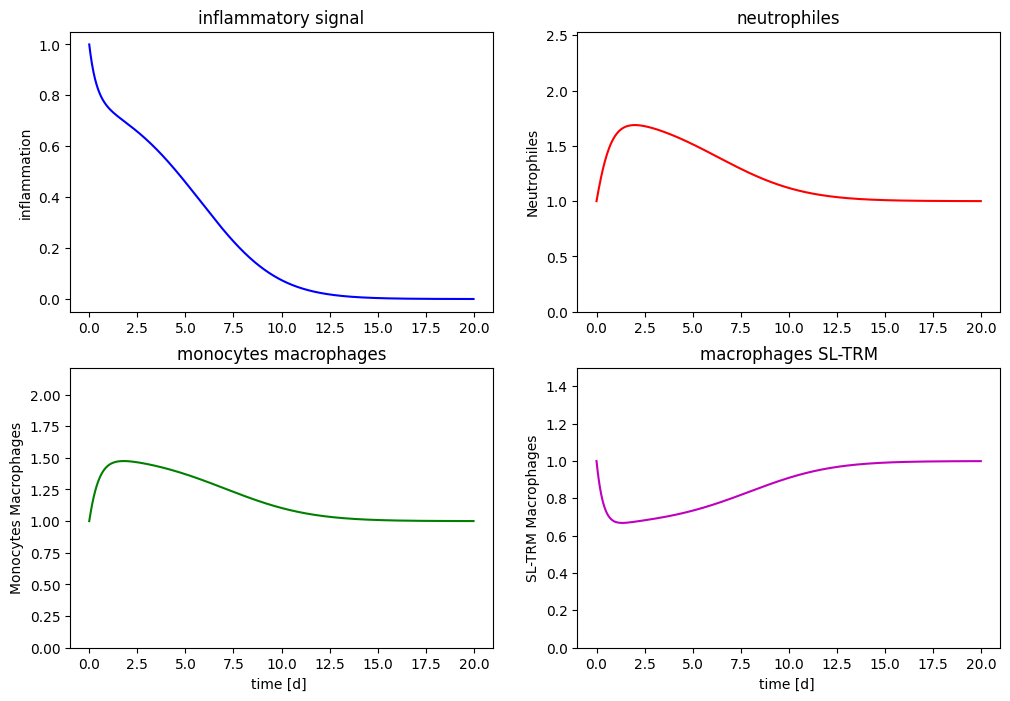
\includegraphics[width=.7\textwidth]{A=0,35.png}
    \caption{A=0.35}
    \label{035}
\end{figure}
Now let us take $a=0.38$, keeping the other parameters unchanged.
\begin{figure}[htbp]
    \centering
    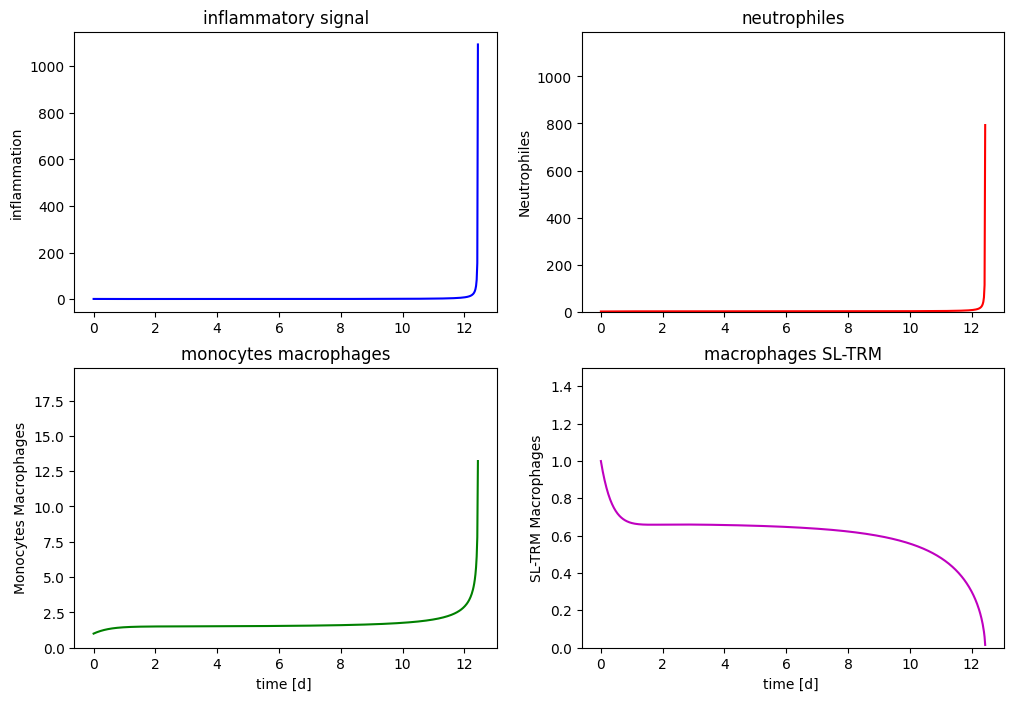
\includegraphics[width=.7\textwidth]{A=0,38.png}
    \caption{A=0.38}
    \label{038}
\end{figure}
We see clearly  in fig.~\ref{035} that for $A=0.35 < 1$ the system converges to the disease-free equilibrium, whereas for $A=0.38$ the system diverges away from this equilibrium, indicating a chronic inflammatory state, see fig. \ref{038}. 
We can also decrease the initial immune signal $S(0)$ to see if the system converges to the disease-free equilibrium or diverges away from it.
Halving the initial immune signal i.e.taking $S(0)=0.5$ and $A=0.38$, we obtain the following result:
\begin{figure}[htbp]
    \centering
    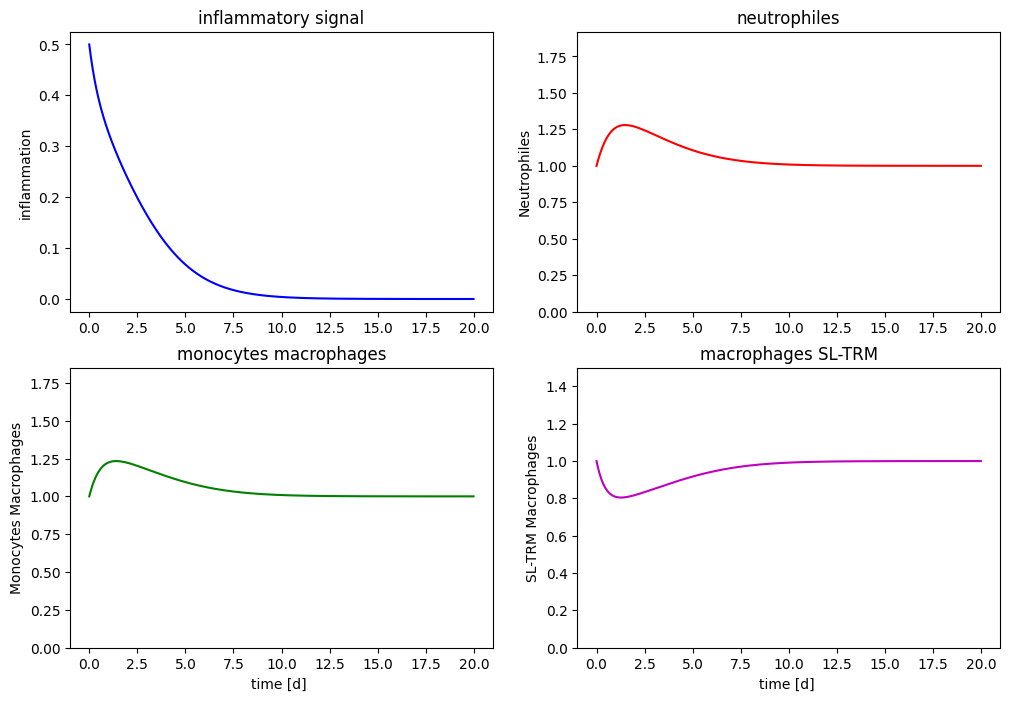
\includegraphics[width=.7\textwidth]{A=0,38_S0=0,5.png}
    \caption{A=0.38, S(0)=0.5}
    \label{038_05}
\end{figure}
We see in fig.~\ref{038_05} that even if $A=0.38$, the system converges to the disease-free equilibrium, indicating that the initial immune signal is not strong enough to trigger a chronic inflammatory state.
We can also start from a depressed immunitory state, taking $S(0)=0.5, N(0)=1, M(0)=0.1, T(0)=0.05$ and $A=0.38$. We observe in fig. \ref{038_depressed} that the system diverges away from the disease-free equilibrium, indicating a chronic inflammatory state, even if the initial immune signal is low.
\begin{figure}[htbp]
    \centering
    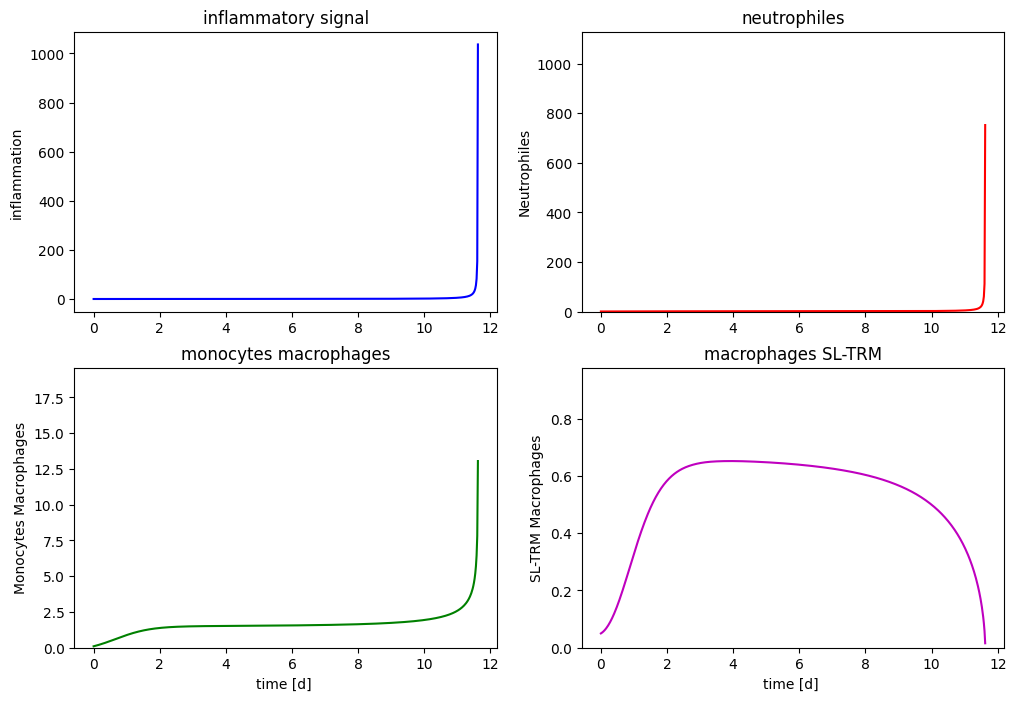
\includegraphics[width=.7\textwidth]{A=0,38_S0=0,5_M=0,1_T=0,05.png}
    \caption{A=0.38, depressed initial conditions}
    \label{038_depressed}
\end{figure}
\begin{figure}[htbp]
    \centering
    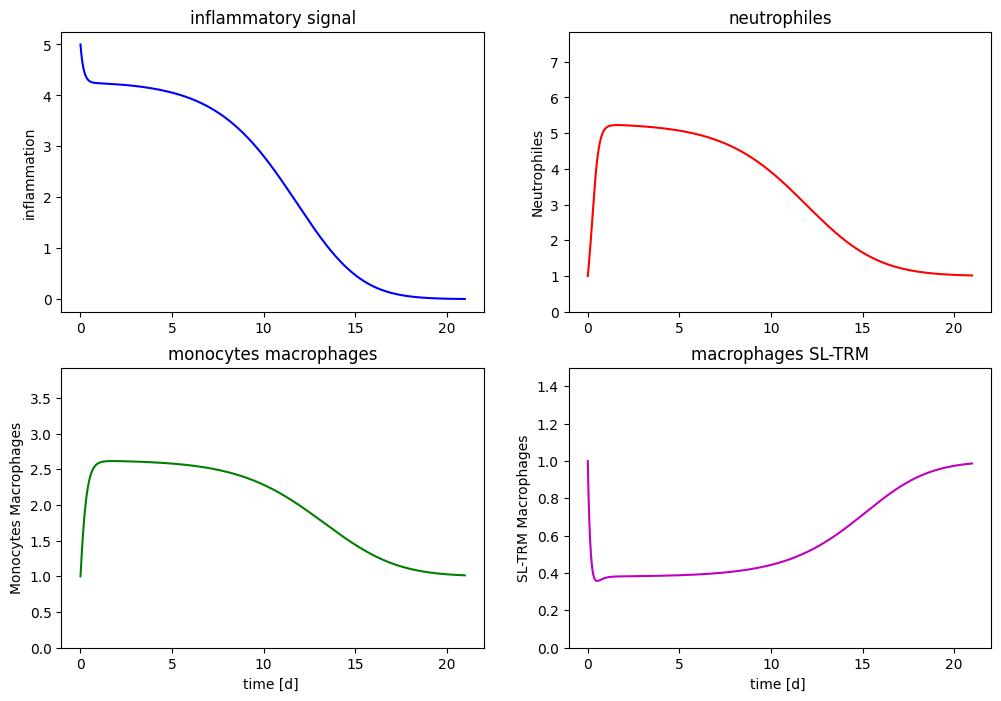
\includegraphics[width=.7\textwidth]{A=0,072_S0=5.png}
    \caption{A=0.072, S(0)=5}
    \label{A=0,072}
\end{figure}
We can also start from a very high initial immune signal, taking $S(0)=5, N(0)=1, M(0)=1, T(0)=1$ and $A=0.072$. We observe in fig. \ref{A=0,072} that the system returns to the disease-free equilibrium, indicating that even if the initial immune signal is high, the system can still heal when $A=0.072 < 1$.
But if we slightly increase $A$ to $A=0.073$, keeping the other parameters unchanged, we observe in fig. \ref{A=0,073} that the system diverges away from the disease-free equilibrium, indicating a chronic inflammatory state.
\begin{figure}[htbp]
    \centering
    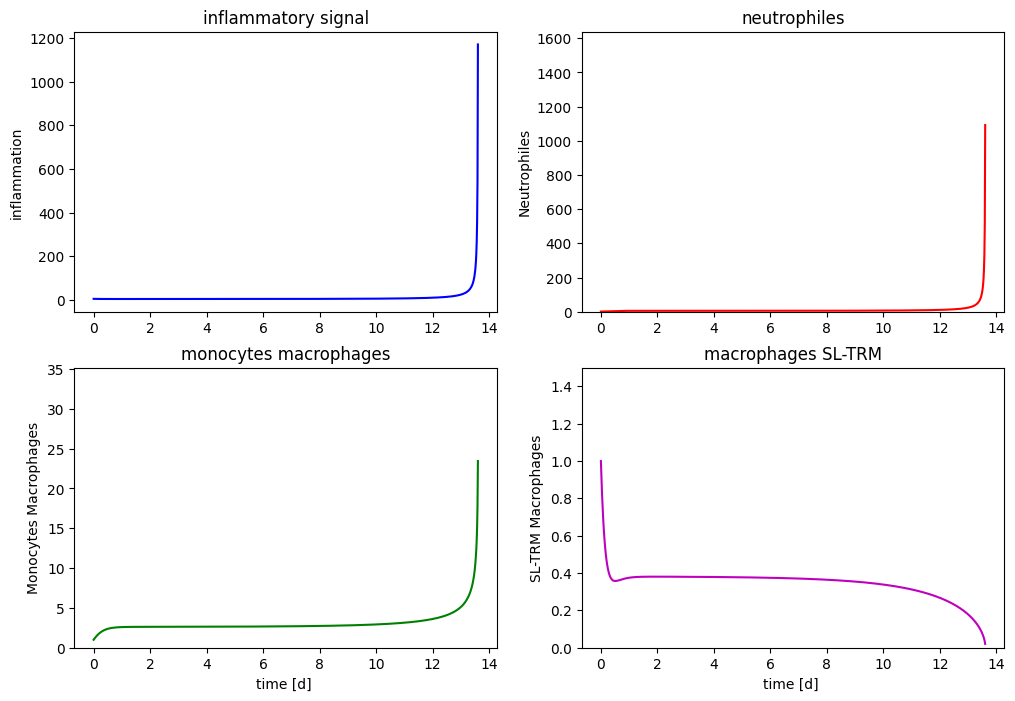
\includegraphics[width=.7\textwidth]{A=0,073_S0=5.png}
    \caption{A=0.073, S(0)=5}
    \label{A=0,073}
\end{figure}
To see how the parameter $A=a/b$ controls the healing prognosis
we plot in Fig. \ref{heal} a $(A,S)$ plane figure where for each value of $A$ and starting value $(S(0)=S,N=1,M=1,T=1)$
 we run the model for three weeks and see how far from the disease-free state the systems ends up.
 We color in green points where $(S,M,N,T)$ is close to $(0,1,1,1)$ up to a given tolerance (say 5\%).
 We color in red points which end up far away from the equilibrium.
 \begin{figure}[!htbp]
    \centering
    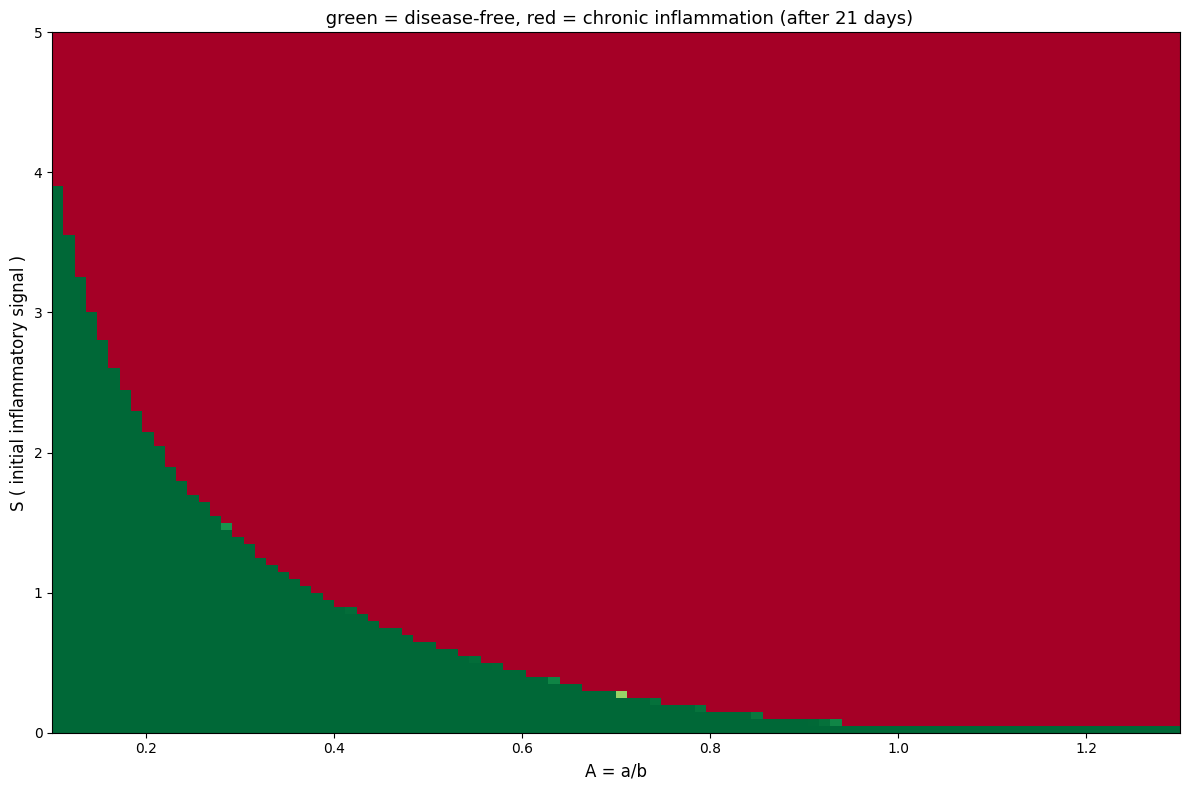
\includegraphics[scale=0.5]{healing.png}
    \caption{Healing w.r.t. $A=a/b$ and initial dose of immune signal $S$}
    \label{heal}
\end{figure}
We notice that for $A<1$, the system converges to the disease-free equilibrium provided that the   initial immune signal $S(0)$ is below a given threshold.
 This threshold increases as $A$ decreases, meaning that the system can tolerate higher initial immune signals without diverging away from the disease-free equilibrium when $A$ is smaller. 
 For $S(0)> 5$, meaning the immune signal dosis is five times the standard value, the system diverges away from the disease-free equilibrium for all values of $A$, 
 indicating a chronic inflammatory state regardless of the value of $A>0$ when the initial immune signal is too high.
For $A>1$, the system diverges away from the disease-free equilibrium for all values of the initial immune signal $S(0)$, indicating a chronic inflammatory state regardless of the initial conditions.
% \mbox{}\\   
% \par\noindent
% We can plot a phase space trajectory in the $(S,N,M,T)$ 4D space, using color intensity to represent the $S$ variable in fig. \ref{phase_space_color}.
% \begin{figure}[!htbp]
%    \centering
 %   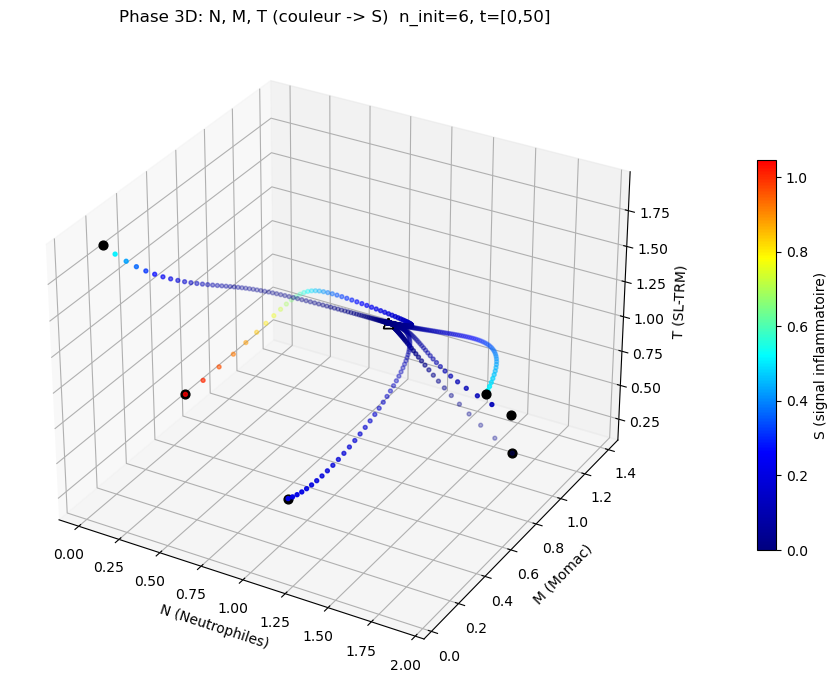
\includegraphics[width=.7\textwidth]{phase_space.png}
%    \caption{Phase space trajectory in the $(S,N,M,T)$ space, $S$ intensity corresponds to the color scale.}
 %   \label{phase_space_color}
%\end{figure}
%\par\noindent
%We can also plot some 2D projections of the 4D phase space trajectory using the tesseract representation in fig. \ref{phase_space_tesseract}.
%\begin{figure}[!htbp]
 %   \centering
 %   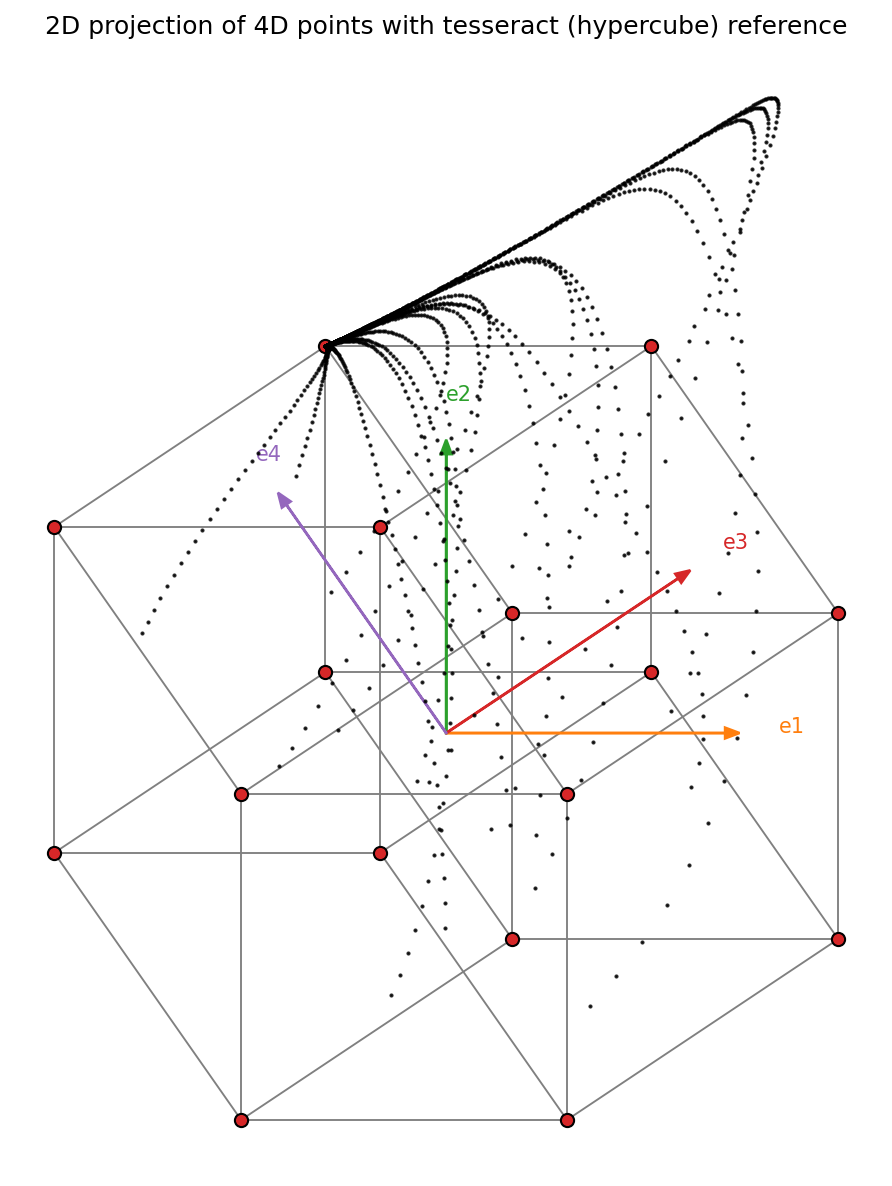
\includegraphics[width=.45\textwidth]{phase_space_tesseract.png}
 %   \caption{2D projections of the 4D phase space trajectory using the tesseract representation.}
 %   \label{phase_space_tesseract}
%\end{figure}
%\bigskip
%\noindent

%\emph{We need to have realistic values for the parameters to feed the model.}

The Python Jupyter notebook used to perform the simulations is available at \url{https://github.com/azerad/immunomath}.
\section{Concluding remarks and perspectives.}\label{sec:conclusion} In this work, we designed a simple model able to describe essential features of the monocyte-macrophages, neutrophiles and sub lining tissue resident macrophages dynamics submitted to an inflammatory stimulus.
We identify a single parameter controlling the positive or negative feedbacks processes at stake in arthritis. 
Essentially it is the ratio between the inflammatory effect of neutrophiles vs the anti-inflammatory effect of SL-TRM macrophages. It suggests that drugs acting \emph{differently} on neutrophiles and SL-TRM macrophages could be effective in curing arthritis.
In future work, we plan to study the effect of such drugs using optimal control theory.




\section*{Acknowledgments}
We acknowledge the support of Immun4Cure University Hospital Institute "Institute for innovative immunotherapies in autoimmune diseases" [France 2030/ANR-23-IHUA-0009].
%\clearpage
% Bibliography réarrangée par ordre chronologique
%\newpage
\begin{thebibliography}{9}
% 2001
\bibitem{seymour2001}
Seymour, R. M. \& Anderson, B. (2001)
\newblock Pro-inflammatory–anti-inflammatory cytokine dynamics
mediated by cytokine-receptor dynamics in monocytes.
\newblock \emph{IMA Journal of Mathematics Applied in Medicine and Biology}, 
  18, 159–192.
\newblock \url{https://doi.org/10.1093/imammb/18.2.159}
% 2005
\bibitem{jit2005}
Jit, M., et al. (2005).% ode compartement
\newblock Mathematical modelling of rheumatoid arthritis.
\newblock \emph{Rheumatology}, 44, 323--331.
\newblock \url{https://doi.org/10.1093/rheumatology/keh491}
% 2007
\bibitem{andrew}
 Andrew, S. M.
Baker, C. T.H.
Bocharov, G. A. (2007)
\newblock Rival approaches to mathematical modelling in immunology
\newblock \emph{Journal of computational and applied mathematics}, 205, p.669--686
\url{https://doi.org/10.1016/j.cam.2006.03.035}

% 2013
\bibitem{baker2013}
Baker, M., et al. (2013).
\newblock Mathematical modelling of cytokine-mediated inflammation in rheumatoid arthritis
\newblock \emph{Mathematical Medicine and Biology}, 30, 311--337. \url{https://doi.org/10.1093/imammb/dqs026}
% 2016
\bibitem{haraux2016}
Haraux A. (2016)
\newblock A simple characterization of positivity preserving semi-linear parabolic systems. 
\newblock \emph{J. Korean Math. Soc.} 54,  1817--1828; MR3718426
\newblock\url{https://doi.org/10.4134/JKMS.j160701}
% 2017
\bibitem{baker2017} %ode compartement
Baker, M., et al. (2017).
\newblock Mathematical modelling of cytokines, MMPs and
fibronectin fragments in osteoarthritic cartilage
\newblock \emph{Journal of Mathematical Biology}, 75, 985--1024 (2017).
\newblock \url{https://doi.org/10.1007/s00285-017-1104-y}

% 2018
\bibitem{zhou2018}
Zhou, X., et al. (2018).% ode compartement
\newblock Circuit Design Features of a Stable Two-Cell System.
\newblock \emph{Cell}, 172, 744--757.
\newblock \url{https://doi.org/10.1016/j.cell.2018.01.015}

% 2019
\bibitem{dsairm2019}
Handel, A. et al. (2019)
\newblock Software DSAIRM: dynamical systems
approach to immune response modeling. GitHub
\newblock\url{https://ahgroup.github.io/DSAIRM/}

\bibitem{friedman}
Moise, N. and Friedman, A. (2019)
\newblock Rheumatoid arthritis, a mathematical model, 
\newblock \emph{J. Theoret. Biol.}, 461, 17--33
\url{https://doi.org/10.1016/j.jtbi.2018.10.039}

\bibitem{jaiani2019}%ode compartement
Odisharia, K.,  Odisharia, V.,  Tsereteli, P., 
and  Janikashvili, N. (2019).
\newblock On the Mathematical Model of Drug
Treatment of Rheumatoid Arthritis
\newblock In
G. Jaiani and D. Natroshvili (eds.).
\newblock Mathematics, Informatics, and their Applications in Natural Sciences and Engineering.
\newblock \emph{Springer Proceedings in Mathematics \& Statistics}, 2019. \url{https://doi.org/10.1007/978-3-030-10419-1_10}

% 2020
\bibitem{Handel2020}%review
Handel, A., et al  (2020).
\newblock Simulation modelling for immunologists
\newblock \emph{Nature Reviews Immunology}, 20, 186--195. \url{https://doi.org/10.1038/s41577-019-0235-3}
% 
\bibitem{macfarlane2020}
 Macfarlane Fiona R.,  Chaplain Mark A. J. \&  Eftimie Raluca (2020).
\newblock Quantitative Predictive Modelling Approaches to
Understanding Rheumatoid Arthritis: A Brief Review
\newblock \emph{Cell}, 9:74 
\url{https://doi.org/10.3390/cells9010074}
% 2022
\bibitem{macfarlane2022} %review
Macfarlane, F. R., Chaplain, M. A. J., \& Eftimie, R. (2022).
\newblock Modelling rheumatoid arthritis: A hybrid model of pannus formation in a small joint.  
\newblock \emph{Immunoinformatics}, 6, 100014 
 \url{https://doi.org/10.1016/j.immuno.2022.100014}

% 2024
\bibitem{frontiers2024} %review
Ugolkov, Y., et al. (2024)
\newblock Mathematical modeling in
autoimmune diseases: from theory to clinical application
\newblock \emph{Frontiers in Immunology}, 15, 1371620. \url{https://doi.org/10.3389/fimmu.2024.1371620}

\bibitem{relouw}
 Relouw Freek J. A.,  van Riel Natal A. W.,  Kox Matthijs,  Taal H. Rob,  Koch Birgit C. P.,  Prins Menno W. J.
(2024)
\newblock Mathematical model of the inflammatory
response to acute and prolonged
lipopolysaccharide exposure in humans
\newblock \emph{npj|Systems Biology and Applications} 10, 146
\url{https://doi.org/10.1038/s41540-024-00473-y}

\bibitem{torres2024}
Ciuperca I, Pujo-Menjouet L,
Matar-Tine L, Torres N, Volpert V. (2024)
\newblock A qualitative analysis of an A$\beta$-monomer model with inflammation processes for Alzheimer’s
disease.
\newblock \emph{R. Soc. Open Sci.}, 11, 231536.
\url{https://doi.org/10.1098/rsos.231536} 

\end{thebibliography}


\end{document}